\chapter{Tworzenie polskich zbiorów}
W szczególności w ostatnim czasie nacisk zostaje przenoszony z modeli na odpowiednie przygotowanie i jakość zbiorów danych. Przykładem tego są wydane w ostatnim czasie artykuły \bibtitle{Textbooks are all you need} \mycite{Gunasekar2023} oraz \bibtitle{Orca 2: Teaching small language models how to reason} \mycite{mitra2023orca}, które demonstrują jak dużą poprawę można uzyskać bez powiększania i komplikowania wykorzystywanego modelu, lecz poprzez stworzenie wysokiej jakości zbioru danych. Jako że dla zadania \code{Text-to-SQL} na moment pisania niniejszej pracy nie istnieją żadne zbiory danych w języku polskim, a także ze względu na duże ich znaczenie, wiele uwagi zostało poświęcone tej kwestii. 

Na początku bieżącego rozdziału omówione zostaną przyjęte założenia dotyczące tworzenia polskich zbiorów, a następnie proces ten zostanie krok po kroku opisany. W pierwszej kolejności przedstawiony będzie sposób wstępnego przetworzenia zbiorów angielskich, a następnie skrypt służący do syntezy zbiorów polskich oraz sposób dokonywania poszczególnych tłumaczeń. Na koniec opracowane zbiory zostaną podsumowane i przeanalizowane.

\section{Przyjęte założenia}
Po przeanalizowaniu różnic między istniejącymi tłumaczeniami zbioru \code{Spider} przystąpiono do zdefiniowania założeń na rzecz opracowanie tłumaczeń polskich. Przyjęte założenia obejmują wykorzystanie tłumaczenia maszynowego, generowanie finalnych zbiorów w sposób skryptowy, tłumaczenie dodatkowo zbiorów pokrewnych oraz zachowanie oryginalnej zawartości baz danych. Każde z tych założeń zostanie uzasadnione w osobnej sekcji.

 
 Pierwszym jest wykorzystanie tłumaczenia maszynowego, zamiast manualnego. Drugi stanowi dynamiczne generowanie finalnych zbiorów zamiast jednorazowego tłumaczenia wszystkich przykładów i udostępnienia jedynie zmodyfikowanej ich wersji. Oba założenia zostaną rozwinięte, uzasadnione i dokładnie przedyskutowane w poniższych dwóch sekcjach.

\subsection{Tłumaczenie maszynowe}
Pomimo wskazanej w sekcji \ref{text:translation-method} dominacji tłumaczenia manualnego nad maszynowym postanowiono wykorzystać to ostatnie. Przyczyn tej decyzji jest kilka. Przede wszystkim w realizację tłumaczenia aktywnie zaangażowana jest tylko jedna osoba, w odróżnieniu od wcześniejszych prac, w których w tym procesie uczestniczyło ich kilka, w tym nawet profesjonalni tłumacze. Drugą przesłanką jest ograniczony czas, ze względu na pracę magisterską, w ramach której niniejszy temat jest realizowany. Ostatecznie jest to zadanie żmudne, a zbiór maszynowy, pomimo niższej jakości, także pozwoli, a nawet da więcej czasu, na wykonanie eksperymentów.

\subsection{Skryptowe generowanie zbiorów}
Wszystkie dotychczasowe tłumaczenia zbioru Spider sprowadzają się jedynie do udostępnienia samych danych, czyli zmodyfikowanej wersji zbioru, bez żadnych dodatkowych skryptów. Wydaje się to wystarczające i dla większości zastosowań w rzeczywistości jest. Taki zbiór stanowi bardzo dobry benchmark służący do porównywania różnych algorytmów, ponieważ nie ma żadnych niedomówień w kwestii jego zawartości.

W niniejszej pracy zaproponowano niespotykane, a przynajmniej nie opisane, we wcześniejszych pracach podejście, które polega na skryptowym generowaniu zbiorów w żądanej konfiguracji. Na początku zostaną one rozbite na elementarne składniki, czyli pytania, zapytania SQL oraz nazwy tabel i kolumn. Następnie, po dokonaniu tłumaczenia indywidualnych elementów, będzie można przeprowadzić ich skryptową syntezę w kompletny zbiór, wybierając przy tym żądany język pytań, język zapytań, czy jedno z przypuszczalnie kilku wariantów nazewnictwa tabel i kolumn. 

Zdecydowano się na wykorzystanie zarysowanej metody przede wszystkim dlatego, że zdekomponowanie zbioru znacznie ułatwia tłumaczenie. Chociażby nazwy tabel i kolumn występują zarówno w pliku schematu i próbkach, więc praca na zbiorze w pierwotnej postaci wymagałaby wprowadzania podobnych zmian w kilku miejscach, co jest niewygodne i wrażliwe na błędy. Przypuszcza się, że autorzy wcześniejszych tłumaczeń również mogli wykorzystać podobną technikę, w szczególności ci, którzy dokonywali tłumaczenia schematu. W ich artykułach nie natrafiono jednak na przesłanki mówiące, że tak właśnie było i przedstawiona w dalszej części pracy metoda jest własnym pomysłem.

Korzystając z opisanej metody można stworzyć kilka mapowań starych nazw tabel i kolumn na nowe i do syntezy wykorzystać to, które w danym przypadku wydaje się najlepsze. Przykładowo bazy mogą zawierać nazwy angielskie, polskie, czy też polskie bez znaków diakrytycznych. Jest to poza zakresem pracy, lecz skrypt, który zostanie opracowany, w dużym stopniu ułatwi dokonywanie tłumaczeń na inne języki, bo wszystkie komponenty zbioru \code{Spider} zostały już rozplątane. Generalnie taka strategia jest bardzo elastyczna i otwiera drogę na nowe eksperymenty.

\subsection{Tłumaczenie zbiorów pokrewnych}
Oprócz przetłumaczenia zbioru \code{Spider} postanowiono dokonać tego również dla czterech zbiorów pokrewnych przedstawionych wcześniej w sekcji \ref{text:related-datasets}. Naturalnym powodem jest chęć zdobycia większej liczby próbek w nadziei, że pozwoli to finalnie wytrenować lepszej jakości modele. Dodatkowe zbiory mogą zostać wykorzystane także do testów. W szczególności \code{Spider-Syn} oraz \code{Spider-DK} pozwolą na testowanie tworzonych algorytmów pod kątem odporności na synonimy oraz znajomości wiedzy domenowej. 

Przetłumaczenie dodatkowych zbiorów jest ułatwione, gdyż ich format jest w dużym stopniu zgodny z formatem zbioru \code{Spider}. Poza tym korzystają z tych samych baz danych, co pozwala uniknąć dodatkowego tłumaczenia nazw schematu. Całość jest ułatwiona ze względu wykorzystanie tłumaczenia maszynowego oraz skryptowej syntezy. Nie znaleziono informacji na temat wcześniejszych prób tłumaczenia tych zbiorów, więc niniejsza praca być może jest pierwsza.

\subsection{Oryginalna zawartość baz danych}
Zawartość baz danych postanowiono pozostawić bez zmian -- ewentualnemu tłumaczeniu podlegać będzie jedynie ich schemat. Powodem tego jest duża ilość znajdujących się tam informacji, których tłumaczenie jest kłopotliwe, a także względnie niewielkie korzyści z tego płynące. Jest to jednocześnie zgodne z większością istniejących podejść do tworzenia przekładów zbioru \code{Spider}. Modele trenowane na nich wciąż są w stanie osiągać wysokie wyniki, co potwierdza słuszność takiego podejścia.

Rozważano dokonanie tłumaczenia z wykorzystaniem narzędzi działających offline, by uniknąć wysokich kosztów, lecz nie rozwiązuje to wszystkich problemów. W bazach znajduje się wiele informacji, które należałoby spolszczyć, a tłumacze maszynowe tego nie dokona, czego przykładami są imiona, nazwiska, adresy i skrótowe nazwy. Poza tym wartości występują również w zapytaniach SQL i konieczna by była ostrożność, aby odpowiednie wartości z baz oraz zapytań zostały zgodnie przetłumaczone.

\section{Przygotowanie zbiorów angielskich}
Poza angielskim zbiorem \code{Spider}, którego przetłumaczenie bez wątpienia jest najistotniejsze, powzięto również tłumaczenie zbiorów \code{Spider-Syn}, \code{Spider-DK}, \code{SParC} oraz \code{CoSQL}. Ich struktura nieco odbiega od zbioru \code{Spider}, więc konieczne okazało się wykonanie dodatkowych kroków, które zostały w niniejszej części podsumowane. Niektóre z nich są konieczne, tak jak zamiana zbiorów z kontekstowych na bezkontekstowe, a inne opcjonalne, jak przeprowadzenie deduplikacji. Sprawiają one, że tłumaczenia owych dodatkowych zbiorów nie stanowią idealnych odpowiedników oryginałów. W różnym stopniu, ale należy traktować je jako nowe zbiory i unikać zestawiania osiąganych na nich rezultatów z angielskimi odpowiednikami.

\subsection{Konwersja zbiorów kontekstowych na bezkontekstowe}
W ramach realizowanego tematu rozważany jest problem tłumaczenia bezkontekstowego, co jest pozornie sprzeczne z wykorzystaniem zbiorów \code{SParC} oraz \code{CoSQL}. Nie zawierają one bowiem prostego szeregu pytań i odpowiadających im zapytań SQL, lecz dodatkowo porządkują je w konwersacje, gdzie kolejne wiadomości bazują na znajomości poprzednich. Zauważono jednak, że zbiory kontekstowe mogą zostać przekształcone na bezkontekstowe poprzez przefiltrowanie polegające na wybraniu z każdej konwersacji jedynie pierwszego pytania i odpowiedzi. Nie istnieje wówczas żadna historia wiadomości wcześniejszych, więc takie przykłady nie posiadają kontekstu. Powstałe w ten sposób zbiory znacznie różnią się od oryginalnie kontekstowych \code{SParC} oraz \code{CoSQL}, więc całkowicie nieuzasadnionym jest porównywanie ze sobą osiąganych na nich wyników.

\subsection{Modyfikacja pytań}
Część pytań wewnątrz zamienionych na bezkontekstowe zbiorów \code{SParC} oraz \code{CoSQL} wyraźnie odróżnia się od reszty. Zawierają bowiem wyrażenia charakterystyczne dla konwersacji, takie jak \textit{Hi}, \textit{Hello}, \textit{How are you}. Przykładem jest pytanie \enquote{Hello, how many total documents are there?}. Wymienione wyrażenia są dla rozważanego problemu niepożądane, gdyż nie stanowią typowych zapytań, jakie użytkownik wprowadziłby do systemu, wiedząc, że zwraca jedynie zapytania SQL. Z tego względu znaleziono takie przypadki za pomocą wyrażeń regularnych oraz funkcji wyszukiwania, dostępnej w wykorzystywanym edytorze i usunięto z pytań niechciane początki.

\subsection{Deduplikacja w obrębie zbiorów}
Za zduplikowane zostały uznane przykłady, które posiadają takie same bazy danych oraz znormalizowane angielskie pytania (przekonwertowane na małe litery i bez niepotrzebnych białych znaków). Deduplikacji w obrębie zbiorów dokonano poprzez zwyczajne usunięcie występujących kilkukrotnie próbek. Okazało się, że znaleziono takie w każdym ze zbiorów, poza \code{Spider-DK}. 25 przypadków zostało zlokalizowanych nawet w samym zbiorze \code{Spider}, lecz w nim modyfikacji nie wprowadzano, bo ze względu na jego wysoką renomę chciano, by próbki w polskim wariancie dokładnie mu odpowiadały. Najwięcej duplikatów zostało znalezionych w zbiorze \code{SParC}. Widocznie w tym oryginalnie kontekstowym zbiorze wiele konwersacji rozpoczynało się od tych samych wiadomości i różnice następowały dopiero później.

\subsection{Deduplikacja pomiędzy zbiorami}
Kolejnym problemem okazały się duplikaty występujące pomiędzy zbiorami. W większości występowały one między \code{Spider} a całą resztą, ponieważ \code{Spider} powstał jako pierwszy. Widać to doskonale na rysunku \ref{fig:deduplication-before}, gdyż największa liczba duplikatów znajduje się w wierszu oraz kolumnie odpowiadającej właśnie zbiorowi \code{Spider}. Dużą liczbą powtórzeń wyróżnia się w szczególności para zbiorów \code{Spider} oraz \code{Spider-Syn}, ponieważ w tym ostatnim autorzy umieszczali oryginalną próbkę, jeżeli nie udało im się wymyślić rozsądnego synonimu. Ostatecznie całą duplikację ze zbiorem \code{Spider} postanowiono usunąć. Jedynym wyjątkiem są powtórzenia pomiędzy parą \code{Spider-DK} oraz \code{Spider}, które pozostawiono, ponieważ \code{Spider-DK} ma charakter czysto walidacyjny i 206 znalezionych duplikatów to nie przypadkowe próbki, lecz precyzyjnie wyselekcjonowane ze zbioru \code{Spider} przykłady zawierające wiedzę domenową. Pozostawioną w zbiorach duplikację, po usunięciu części próbek, przedstawiono na rysunku \ref{fig:deduplication-after}. 

\begin{figure}[ht!]
\centering
\begin{subfigure}{0.49\textwidth}
    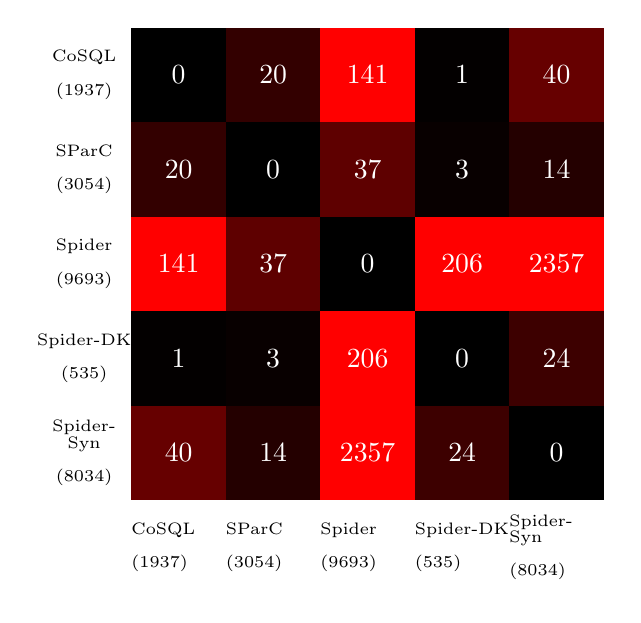
\begin{tikzpicture}[scale=1.2]
      \foreach \y [count=\n] in {
          {0,20,141,1,40},
          {20,0,37,3,14},
          {141,37,0,206,2357},
          {1,3,206,0,24},
          {40,14,2357,24,0},
        } {
          % tiles
          \foreach \x [count=\m] in \y {
            \node[fill=red!\x!black, minimum size=1.2cm, text=white] at (\m,-\n) {\x};
          }
        }
    
      % labels
      \foreach \a [count=\i] in {\code{CoSQL}\\(1937),\code{SParC}\\(3054),\code{Spider}\\(9693),\code{Spider-DK}\\(535),\code{Spider-Syn}\\(8034)} {
        \node[text width=1.2cm,minimum size=1.2cm] at (\i, -6) {\fontsize{6pt}{6pt}\selectfont\makecell{\a}};
        \node[text width=1.2cm, align=center,minimum size=1.2cm] at (0,-\i) {\fontsize{6pt}{6pt}\selectfont\makecell{\a}};
      }
    \end{tikzpicture}
    \caption{Przed deduplikacją}
    \label{fig:deduplication-before}
\end{subfigure}
\hfill
\begin{subfigure}{0.49\textwidth}
    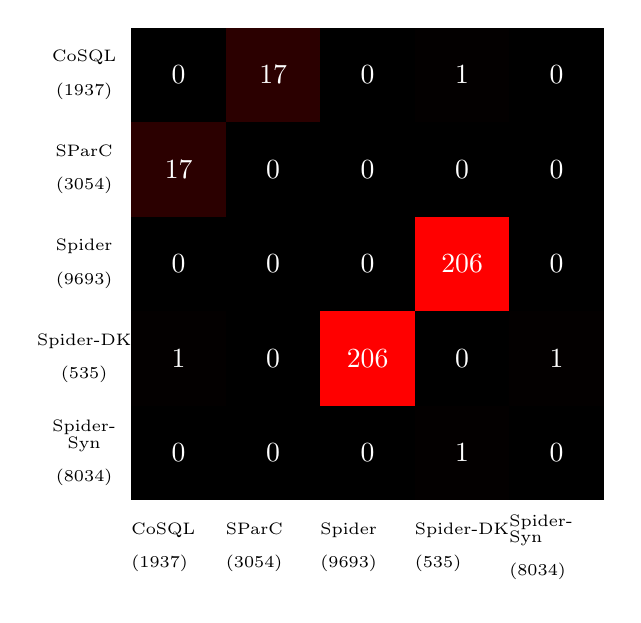
\begin{tikzpicture}[scale=1.2]
      \foreach \y [count=\n] in {
          {0,17,0,1,0},
          {17,0,0,0,0},
          {0,0,0,206,0},
          {1,0,206,0,1},
          {0,0,0,1,0},
        } {
          % tiles
          \foreach \x [count=\m] in \y {
            \node[fill=red!\x!black, minimum size=1.2cm, text=white] at (\m,-\n) {\x};
          }
        }
    
      % labels
      \foreach \a [count=\i] in {\code{CoSQL}\\(1937),\code{SParC}\\(3054),\code{Spider}\\(9693),\code{Spider-DK}\\(535),\code{Spider-Syn}\\(8034)} {
        \node[text width=1.2cm,minimum size=1.2cm] at (\i, -6) {\fontsize{6pt}{6pt}\selectfont\makecell{\a}};
        \node[text width=1.2cm, align=center,minimum size=1.2cm] at (0,-\i) {\fontsize{6pt}{6pt}\selectfont\makecell{\a}};
      }
    \end{tikzpicture}
    \caption{Po deduplikacji}
    \label{fig:deduplication-after}
\end{subfigure}
\lcaption{Diagramy ilustrujące liczbę duplikatów pomiędzy zbiorami}{Na osiach umieszczono nazwy zbiorów wraz z liczbą próbek, a wartości w komórkach macierzy wskazują liczbę duplikatów pomiędzy daną parą zbiorów.}
\label{fig:cross-dataset-duplicates}
\end{figure}

\subsection{Dodatkowa deduplikacja tłumaczeń}
Trzeba zauważyć, że opisane powyżej usuwanie duplikatów bazuje na angielskich wersjach pytań, co wydaje się wystarczające, ponieważ jeżeli pytania angielskie się różnią, to ich polskie tłumaczenia również powinny się różnić. W przypadku próbek zawartych w zbiorze \code{Spider-Syn} jest jednak często inaczej. Dla przypomnienia, zawiera on próbki z oryginalnego zbioru \code{Spider}, lecz z wybranymi słowami zamienionymi na synonimy. Okazuje się, że te synonimy oraz bazowe słowa, od których pochodzą, tłumaczone są niejednokrotnie przez tłumacza maszynowego na te same polskie wyrażenia, co skutkuje duplikatami w liczbie 1350. Proces ich powstawania został zilustrowany na rysunku \ref{fig:deduplication-after-translation}. Aby pozbyć się tak powstałej duplikacji postanowiono usunąć niepotrzebne próbki ze zbioru \code{Spider-Syn}. Działanie to, w odróżnieniu od wcześniej opisanych, musiało się odbyć już po dokonaniu tłumaczenia na język polski.

\begin{figure}[ht!]
  \centering
  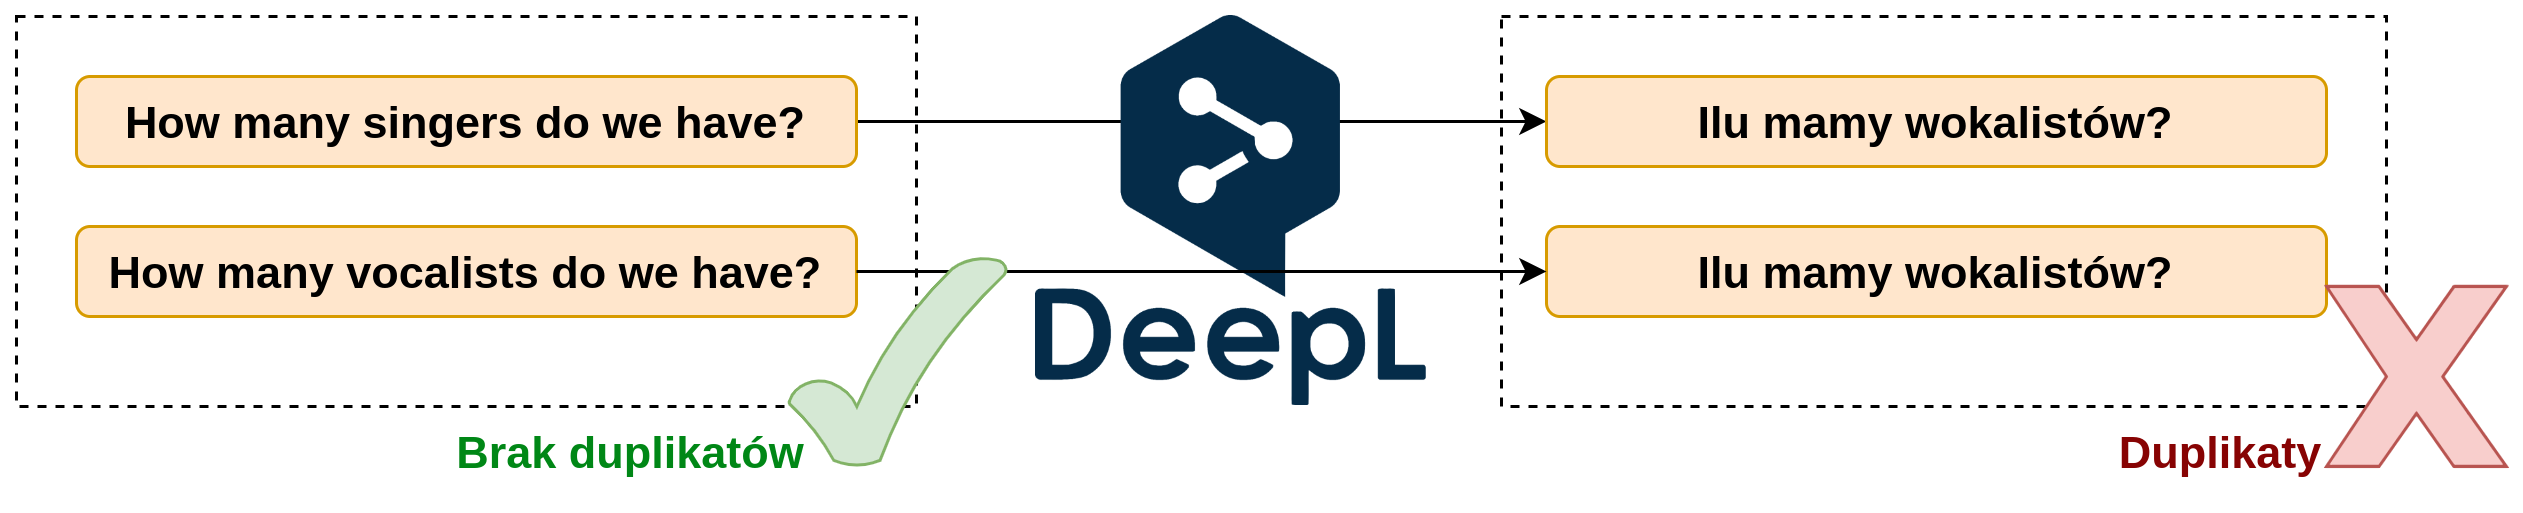
\includegraphics[width=1.0\linewidth]{images/duplication_after_translation.png}
  \caption[Sposób powstawania duplikacji w wyniku tłumaczenia]{Sposób powstawania duplikacji pomiędzy \code{Spider} i \code{Spider-Syn} w wyniku tłumaczenia}
  \label{fig:deduplication-after-translation}
\end{figure}

\section{Skryptowe generowanie zbiorów}
Skryptowe generowanie zbiorów danych jest ważnym elementem niniejszej pracy, który nie został w istniejącej literaturze napotkany. Z tego względu proces ten zostanie w poniższych sekcjach dokładnie opisany. Na początku przedstawione będą dane źródłowe, które niezbędne są w celu przeprowadzenia generacji. W dalszej kolejności omówiony zostanie algorytm służący do mapowania starych nazw schematu na nowe, a na koniec sposób rekonstrukcji redundantnych informacji, które zostały wcześniej usunięte w celu uproszczenia przetwarzania.

\subsection{Dane źródłowe}
Przed przystąpieniem do tworzenia skryptu generującego zbiory konieczne okazało się zastanowienie nad danymi źródłowymi, których on potrzebuje. Zdecydowano się rozbić je na dwie grupy: próbki, zawierające pytania i zapytania SQL w różnych językach oraz mapowania nazw schematu, zawierające kompletne odwzorowania oryginalnych nazw tabel i kolumn na nowe. Informacje te postawiono przechowywać w osobnych plikach JSON, których format zostanie dalej opisany. Taka dekompozycja umożliwia dodawanie kolejnych zbiorów poprzez tworzenie nowych plików próbek i umożliwianie innych sposobów tłumaczenia nazw tabel i kolumn poprzez tworzenie kolejnych plików mapowania.

\subsubsection{Plik próbek}
Plik próbek zawiera listę obiektów JSON, z których każdy reprezentuje konkretny przykład. Jeden z nich przedstawiono na rysunku \ref{lst:new-sample}. Zawiera jedynie niezbędne informacje, czyli nazwę bazy danych oraz alternatywne warianty pytań i zapytań SQL. Posiada angielskie i polskie ich wersje, ponieważ takie są istotne dla realizacji niniejszej pracy. Nic nie stoi jednak na przeszkodzie, aby dodać więcej języków, gdyż zarówno format omawianego pliku, jak i reszta komponentów, zostało na taką okoliczność przygotowane.

\begin{minipage}{\linewidth}
\lstinputlisting[
style=json,
caption=Obiekt JSON z pliku próbek reprezentujący jeden przykład,
label={lst:new-sample},
]{listings/new_sample.json}
\end{minipage}

Warto zwrócić uwagę na fakt, że próbki w pełnym zbiorze posiadają znacznie więcej atrybutów niż te przedstawione powyżej. Zawierają dodatkowo pytania i zapytania SQL podzielone na tokeny oraz sparsowane zapytania. Są to jednak w dużej części informacje redundantne, które można z powodzeniem odtworzyć na podstawie skromnych informacji przedstawionych powyżej i jest to rzeczywiście jedna z funkcji realizowanych przez skrypt generujący. Odtworzenie danych redundantnych niestety wymaga napisania dodatkowego kodu oraz dodaje narzut czasowy do procesu generacji. Z drugiej strony mocno upraszcza dane źródłowe, co jest znacznie ważniejsze biorąc pod uwagę cel, którym jest dokonanie tłumaczenia. 

\subsubsection{Plik mapowania nazw}
Aby umożliwić dokonywanie różnych tłumaczeń schematów baz danych, czyli nazw tabel i kolumn, opracowany został format pliku przedstawiony na listingu \ref{lst:new-trans}. Zawiera on informacje pozwalające na dokonanie mapowania oryginalnych nazw na dowolne inne. Jest to plik JSON o kilku stopniach zagnieżdżenia. Na najwyższym poziomie jest słownikiem, który dla każdej nazwy bazy danych zawiera listę tabel, a każda tabela listę kolumn. Wszystkie obiekty reprezentujące tabele i kolumny posiadają nazwy źródłowe oraz docelowe, na które powinny zostać przetłumaczone. Jak już wiadomo, mają one dwa rodzaje nazw, które zostały tutaj uwzględnione: oryginalnie występujące w bazach danych oraz odpowiedniki w języku naturalnym.

\begin{minipage}{\linewidth}
\lstinputlisting[
style=json,
caption=Fragment opracowanego pliku mapowań nazw schematu,
label={lst:new-trans},
]{listings/new_trans.json}
\end{minipage}

Należy zwrócić uwagę na to, że zaproponowany format pozwala, aby dana nazwa kolumny była tłumaczona na różne sposoby w zależności od tabeli i bazy, w której się znajduję. Podobnie ta sama nazwa tabeli może być tłumaczona na różne sposoby w zależności od zawierającej ją bazy danych. Jest to celowy zabieg i wymagany w celu umożliwienia prawdziwie wysokiej jakości tłumaczenia. Rozważmy dla przykładu tabelę o nazwie \code{department}. W bazie dotyczącej biznesu prawdopodobnie powinna zostać przetłumaczona jako \code{dział}, natomiast w domenie uniwersyteckiej jako \code{wydział}. Przyjęcie przedstawionej struktury pliku mapowania nazw umożliwiło dokonanie tego typu kontekstowych tłumaczeń, co zostało wykorzystane w dalszej części pracy.

\subsection{Zmiana nazw tabel i kolumn}
Zmiana nazw tabel i kolumn zgodnie z opisanym wyżej plikiem mapowania to dla opracowanego procesu generacji zbiorów najważniejszy punkt. Sprowadza się do dokonania modyfikacji w dwóch miejscach. Podmiana nazw w samych bazach danych \code{SQLite} jest prostszą częścią. Znacznie trudniejsze okazuję się dokonanie zmian w zapytaniach. Powstały one przecież na bazie oryginalnych nazw tabel i kolumn, które należy wychwycić i podmienić na nowe.

\subsubsection{Zmiana nazw w bazach danych}
Zmodyfikowanie nazw tabel i kolumn w bazach danych nie stanowi dużego wyzwania, ponieważ wystarczy wykonać na każdej z nich serię instrukcji SQL typu \sql{ALTER TABLE}. Ułatwia to fakt, że język Python posiada w ramach biblioteki standardowej pakiet pozwalający na pracę z bazami \code{SQLite}. Przystępując do tego należy jednak mieć pewność, że zastosowanie danego mapowania nie tworzy konfliktujących ze sobą pod względem nazw elementów, bo wówczas operacja się nie powiedzie. Zadbano o ten aspekt podczas opisanego w dalszej części tłumaczenia pliku mapowań nazw. Podczas implementacji tego etapu zauważono, że należy ignorować tabele \code{sqlite\_sequence}, ponieważ jest to specjalna tabela i modyfikacja jej nazwy nie jest możliwa.

% Aby to sprawdzić oraz zlokalizować miejsca ewentualnych kolizji stworzony został skrypt, który analizuje podane mapowanie pod tym kątem. 

\subsubsection{Zmiana nazw w zapytaniach}
Dokonanie podmiany nazw tabel i kolumn w zapytaniach SQL stanowi najtrudniejszy etap w całym procesie generowania zbiorów. Przyczyną tego jest przyjęte podejście polegające na tym, że dana kolumna może być przetłumaczona na różne sposoby w zależności od tabeli, w której się znajduję. W przypadku modyfikacji baz danych było oczywistym, do której tabeli należy każda kolumna, bo wynika to z ich jasno zdefiniowanej struktury. Zapytania SQL są natomiast w gruncie rzeczy zwykłym tekstem, więc wydobycie z nich kolumn oraz ustalenie powiązanych tabel stanowi niemałe wyzwanie.

Najłatwiejsze podejście do przedstawionego problemu, ale posiadające istotną słabość, wykorzystuje parsowanie zapytań do postaci drzew \code{AST} z wykorzystaniem przedstawionej wcześniej biblioteki \code{SQLGlot}. Na poziomie drzewa można łatwo dokonać modyfikacji wszystkich nazw, bo ustalenie przynależności kolumn do tabel jest znacznie prostsze ze względu na jego hierarchiczną strukturę. Po modyfikacji drzewa należy zrekonstruować na jego podstawie zapytanie SQL, do którego wprowadzone zmiany się przeniosą. Jak zostało sprawdzone, taka strategia rzeczywiście pozwala na skuteczne przetłumaczenie nazw schematu, jednak wspomnianą słabością jest to, że przetworzone zapytania różnią się delikatnie od oryginałów pod względem formatowania oraz struktury. Powodem są następujące po sobie etapy parsowania i rekonstrukcji z wykorzystaniem biblioteki \code{SQLGlot}, które zachowują jedynie znaczenie zapytań, pozwalając sobie przy tym na delikatne modyfikacje zapisu. Zostało to przedstawione na rysunku \ref{fig:sqlglot-translation}. Przetłumaczone zapytania odbiegają więc nadmiernie od pierwotnych i porównywanie stworzonego tak zbioru z oryginalnym mogłoby być kwestionowane. W szczególności wiele algorytmów opiera się na specyficznym dla poszczególnych zbiorów formacie zapytań i jego modyfikacja mogłaby doprowadzić do problemów z uruchomieniem części modeli. Z przytoczonych powodów takie podejście zostało porzucone.

% listing
\begin{figure}[ht!]
\centering
\begin{subfigure}{0.48\textwidth}
    \begin{minipage}{\linewidth}
        \lstinputlisting[
        style=sql,
        numbers=none,
        escapechar=@,
        nolol,
        ]{listings/sqlglot_before.sql}
    \end{minipage}
    \caption{Zapytanie pierwotne}
    \label{fig:sqlglot-before}
\end{subfigure}
\hfill
\begin{subfigure}{0.48\textwidth}
    \begin{minipage}{\linewidth}
        \lstinputlisting[
        style=sql,
        numbers=none,
        escapechar=@,
        nolol,
        ]{listings/sqlglot_after.sql}
    \end{minipage}
    \caption{Zapytanie zmodyfikowane}
    \label{fig:sqlglot-after}
\end{subfigure}
\lcaption{Przykład drobnych modyfikacji wprowadzanych przez bibliotekę \code{SQLGlot}}{Zapytanie po prawej stronie powstało przez sparsowanie lewego do drzewa \code{AST} i powrót do postaci SQL.}
\label{fig:sqlglot-translation}
\end{figure}

W celu przetłumaczenia nazw w zapytaniach, bez niepotrzebnego wpływania na strukturę, zdecydowano się ostatecznie zrobić to na niższym poziomie. Opracowany został skomplikowany algorytm, który dokonuje tokenizacji zapytań, a następnie analizuje wszystkie tokeny po kolei i jeżeli wykryje nazwę tabeli bądź kolumny to podmienia ją na nową. Aby sprawdzić, czy dany token jest nazwą, dokonywano parsowania zapytania do drzewa \code{AST}, następnie modyfikowano token na inny i ponownie parsowano zapytanie do \code{AST}. Porównując ze sobą tak powstałe drzewa, można ustalić, czy zmodyfikowanym tokenem jest nazwa tabeli, nazwa kolumny, czy żadne z powyższych. W przypadku nazw kolumn konieczne jest dodatkowe ustalenie przynależności do tabeli. Wyróżniono tutaj trzy przypadki:

\begin{enumerate}
    \item Nazwa kolumny poprzedzona nazwą tabeli (\sql{SELECT order.id FROM order})
    \item Nazwa kolumny poprzedzona aliasem (\sql{SELECT T1.id FROM order as T1})
    \item Nazwa kolumny bez tabeli (\sql{SELECT id FROM order})
\end{enumerate}

Pierwszy scenariusz jest najprostszy, ponieważ nazwa tabeli jest jawnie podana i nie ma co do niej wątpliwości. Drugi przypadek jest bardziej skomplikowany, gdyż zamiast istniejącej nazwy tabeli wykorzystany zostaje alias, więc wcześniej trzeba wydobyć z zapytania wszystkie aliasowania. Trzeci przypadek jest również trudny, ponieważ kolumna należy do jednej z wykorzystanych w zapytaniu tabel, więc trzeba wiedzieć dodatkowo, jakie tabele są dostępne. Dla tych dwóch przypadków sytuację dodatkowo komplikuje fakt, że zapytania mogą być swobodnie zagnieżdżanie i łączone szeregowo za pomocą operatorów zbiorowych, co skutkuje pojawieniem się w obrębie pojedynczych zapytań zakresów, w których dostępne są różne tabele i różne aliasowania. Prosta analiza zbioru \code{Spider} wykazała, że 15,6\% zapytań takie zakresy zawiera. 

Aby poradzić sobie z ustaleniem przynależności kolumn do tabel w skomplikowanych zapytaniach postanowiono dokonywać rekurencyjnego rozbijania składających się na nie tokenów na zapytania prostsze. Przekazywany jest przy tym kontekst mówiący o obowiązującym aliasowaniu z zapytań zewnętrznych do wewnętrznych. Zostało to zilustrowane na rysunkach 
\ref{fig:query-decomposition-serial} oraz \ref{fig:query-decomposition-nested}. Przedstawiają odpowiednio dekompozycję zapytania zawierającego operator zbiorowy oraz dekompozycję zapytania z zagnieżdżeniem. W wyniku takiego rekurencyjnego procesu rozbijania otrzymywany jest zbiór elementarnych zapytań wraz z obowiązującymi wewnątrz nich kontekstami, co pozwala na łatwe przetłumaczenie tokenów będących nazwami tabel i kolumn. Jako, że pierwotnym źródłem tych tokenów jest wejściowe, skomplikowane zapytanie, to również ono jest tłumaczone -- niejako jako efekt uboczny, lecz było to celem od samego początku.

\begin{figure}[ht!]
  \centering
  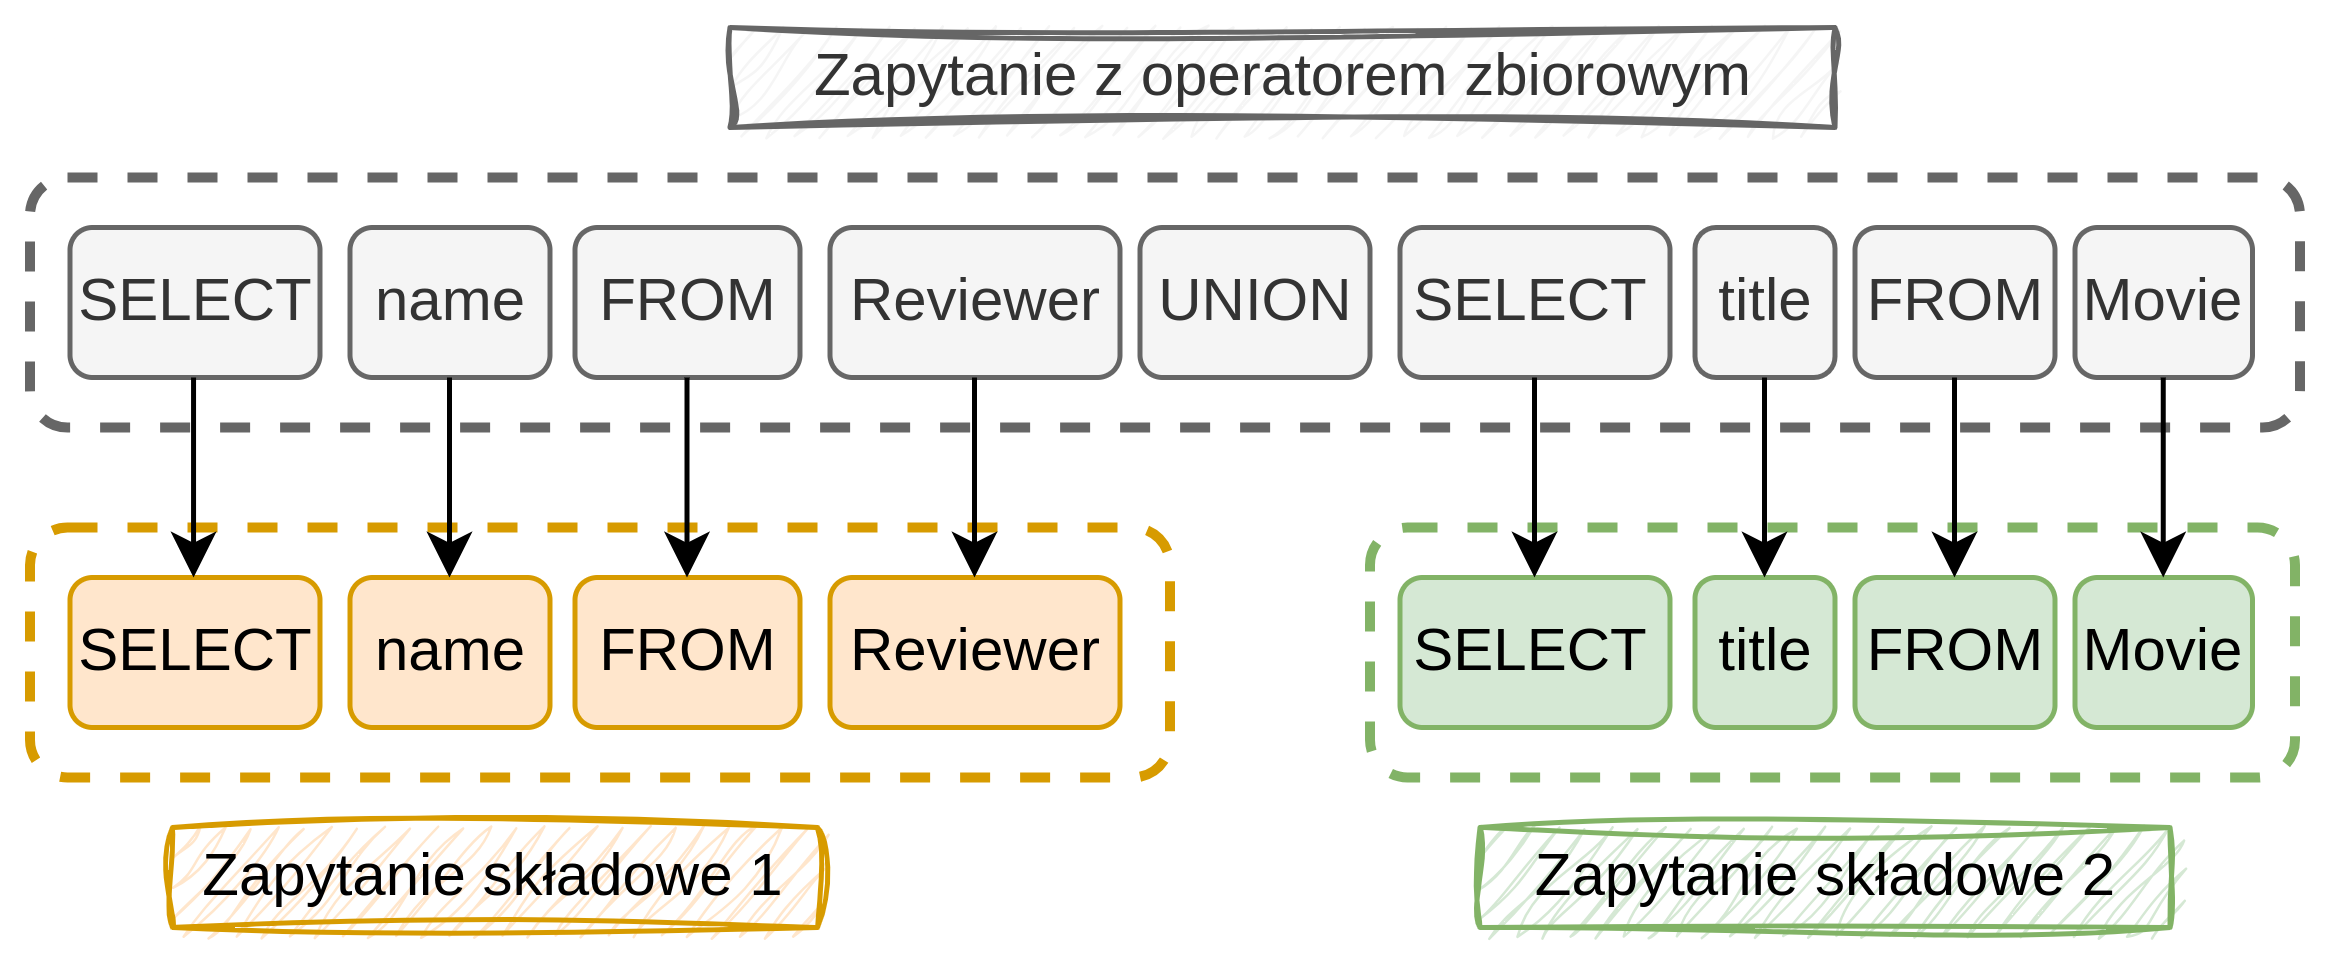
\includegraphics[width=1.0\linewidth]{images/query_decomposition_serial.png}
  \caption{Metoda dekomponowania zapytań z operatorami zbiorowymi}
  \label{fig:query-decomposition-serial}
\end{figure}

\begin{figure}[ht!]
  \centering
  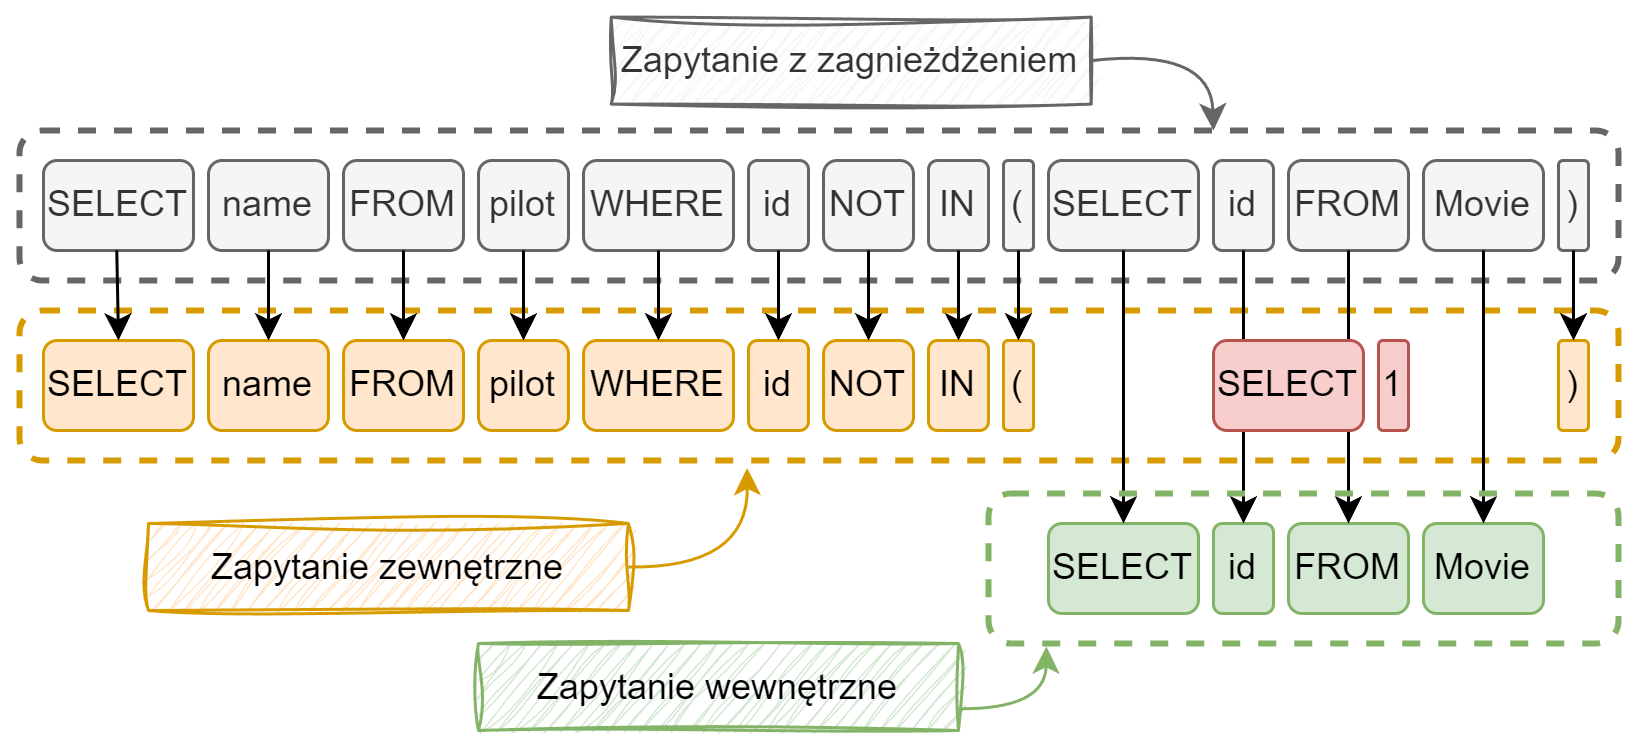
\includegraphics[width=1.0\linewidth]{images/query_decomposition_nested.png}
  \lcaption{Metoda dekomponowania zapytań z zagnieżdżeniem}{Fragment w zapytaniu zewnętrznym odpowiadający zapytaniu wewnętrznemu zastępowany jest wyrażeniem \code{SELECT 1}, aby zapewnić strukturalną poprawność obu rezultatów dekompozycji.}
  \label{fig:query-decomposition-nested}
\end{figure}

\subsection{Rekonstrukcja informacji redundantnych}
Jak zostało wcześniej wskazane, dane źródłowe, na których bazuje algorytm generacji, zawierają jedynie informacje niezbędne. W pełnym zbiorze muszą znaleźć się również te, które zostały uznane za redundantne i w danych źródłowych pominięte. Redundancja ta nie polega na dokładnych powtórzeniach, bo usunięte informacje stanowią pochodne innych. Dokonanie ich rekonstrukcji stanowi sedno niniejszej części.

Znaczną część koniecznych do odtworzenia informacji stanowią pytania i zapytania SQL podzielone na tokeny. Okazuję się jednak, że duża liczba istniejących rozwiązań w ogóle nie korzysta z tych informacji, ponieważ tokenizacji można dokonać na różne sposoby. Zamiast tego wykonują ją samodzielnie, wybierając sposób dla siebie najkorzystniejszy. Niemniej jednak pierwsze modele (najwcześniej opracowane), jak i zapewne część nowszych, korzysta z dostarczonego w ramach zbioru sposobu tokenizacji, więc należy o ten aspekt mimo wszystko zadbać.

\subsubsection{Tokenizacja pytań (atrybut \hcode{question\_toks})}
Pytania podzielone na tokeny powinny znaleźć się w finalnych próbkach pod atrybutem o nazwie \code{question\_toks}. Tokenizacji postanowiono dokonywać z wykorzystaniem dostarczonego w ramach biblioteki \code{SpaCy} wielojęzycznego modelu. Wybrano akurat wariant wielojęzyczny, a nie polski, ponieważ dzięki temu skrypt generujący nie będzie wprowadzał dodatkowych ograniczeń co do języka pytań, a generowanie zbiorów, chociażby z angielskimi pytaniami, również okazało się przydatne. Porównano jednocześnie rezultaty tokenizacji polskich pytań za pomocą modelu wielojęzycznego oraz polskiego. Okazuję się, że wyniki różnią się jedynie w niewielkiej liczbie przypadków, co świadczy o tym, że model wielojęzyczny jest wysokiej jakości.

\subsubsection{Tokenizacja zapytań SQL (atrybut \hcode{query\_toks})}
Zapytania SQL podzielone na tokeny to element, który również musi znaleźć się w kompletnym zbiorze. Występuje w próbkach pod postacią atrybutu \code{query\_toks}. Zaproponowany sposób tokenizacji opiera się na początkowym znalezieniu w zapytaniu wszystkich wartości tekstowych. Wartości te są następnie tokenizowane za pomocą wspomnianego wcześniej wielojęzycznego modelu z biblioteki \code{SpaCy}. Reszta zapytania jest natomiast rozbijana na elementy składowe z wykorzystaniem biblioteki \code{SQLParse}. Proces ten został zilustrowany na rysunku \ref{fig:query-tokenization}.

\begin{figure}[ht!]
  \centering
  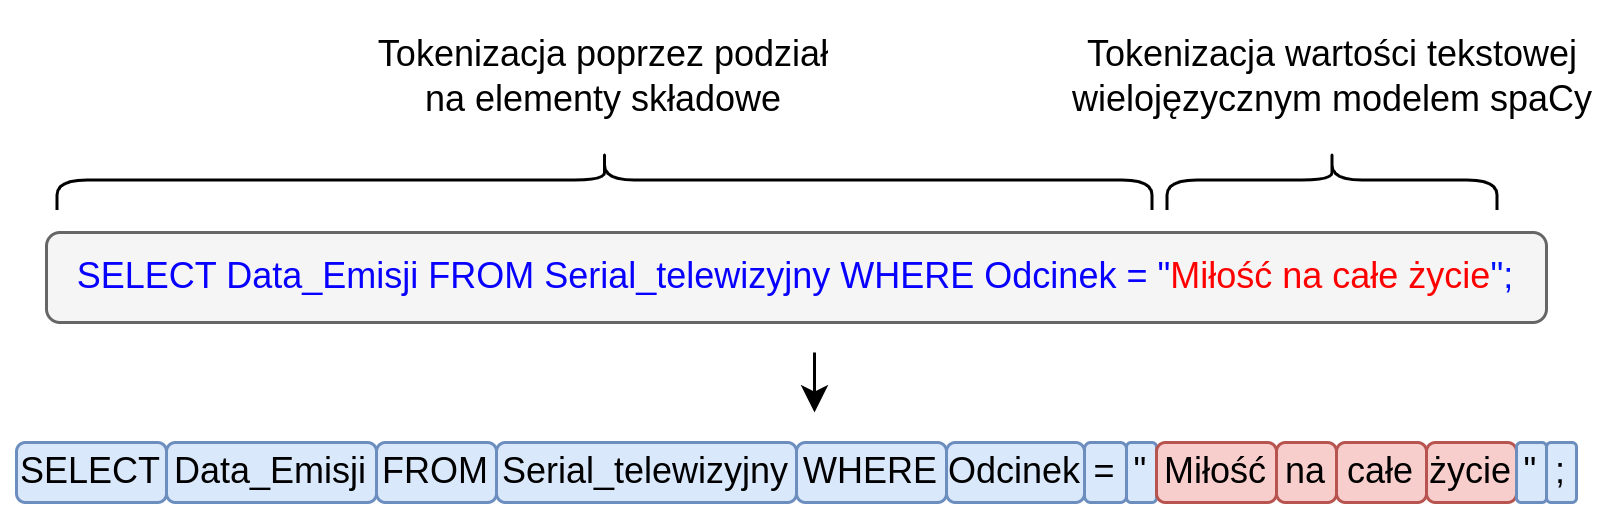
\includegraphics[width=0.9\linewidth]{images/query_tokenization.png}
  \caption{Schemat działania zaproponowanego algorytmu tokenizacji zapytań SQL}
  \label{fig:query-tokenization}
\end{figure}

\subsubsection{Tokenizacja zapytań SQL bez wartości (atrybut \hcode{query\_toks\_no\_value})}
Format zbioru \code{Spider} wymaga od próbek posiadania atrybutu \code{query\_toks\_no\_value}, który musi zawierać zapytanie SQL podzielone na tokeny, lecz bez wartości. Mówiąc bardziej precyzyjnie, wartości powinny zostać zamaskowane za pomocą specjalnego tokena \code{value}. Łatwo zauważyć, że atrybut \code{query\_toks\_no\_value} jest bardzo podobny do opisywanego chwilę wcześniej \code{query\_toks}. Postanowiono więc wykorzystać identyczną technikę, lecz z jedną różnicą: znalezione w zapytaniach wartości, zamiast podlegać rozbiciu na tokeny, są po prostu zastępowane wspomnianym tokenem specjalnym. 

Opracowany algorytm jest niemal całkowicie zbieżny z wykorzystanym w oryginalnym zbiorze \code{Spider} sposobem tokenizacji zapytań. Aby to zweryfikować, dokonano za jego pomocą podziału oryginalnych zapytań i sprawdzono, czy wyniki pokrywają się z oryginalnymi tokenami. Okazuję się, że różnice występują jedynie w 18 przypadkach spośród prawie dziesięciu tysięcy. Dokładniejsza analiza tych kilkunastu przykładów sugeruje, że zapytania SQL w nich zawarte zostały podzielone na tokeny w niekonsekwentny, odbiegający od reszty sposób. Zbiór \code{Spider} nie jest więc do końca spójny. Brak konsekwencji to jeden z problemów, którym rozwijana strategia generowania zbiorów powinna przeciwdziałać i jak widać, ma to rzeczywiście znaczenie.

\subsubsection{Parsowanie zapytań SQL (atrybut \hcode{sql})}
Ważnym elementem, który musi się znaleźć w finalnym zbiorze, są odpowiednio sparsowane zapytania SQL. Mają swoje miejsce w próbkach pod kluczem \code{sql}. Tym razem istnieje publicznie dostępny skrypt, który dokonuje tego procesu. Stanowi go plik \code{parse\_sql.py}, znajdujący się w repozytorium kodu \mycite{spider-repo} dostarczonym przez twórców \code{Spider}. Zostały napotkane jednak pewne problemy wynikające z jego niedociągnięć. W jednym z pierwszych kroków przeprowadza on bowiem operację wydobycia z podanego zapytania aliasowania, czyli słownika mówiącego, jakie występują w nim aliasy i na jakie tabele się mapują. Niestety dokonuje tego globalnie, a jak zostało przedyskutowane wcześniej, nie sprawdza się to dla wszystkich zapytań, ponieważ występują w nich zakresy -- w jednej części zapytania dany alias może mapować się na zupełnie inną tabelę niż w drugiej części. Podczas uruchamiana tego skryptu na zapytaniach ze zbioru \code{Spider}, co jest najczęstszym scenariuszem, nie zwraca żadnych błędów. Przypuszcza się, że kłopotliwe zapytania zostały ręcznie poprawione tak, aby stały się parsowalne. W przypadku gdy jednak zostaną wcześniej poddane tłumaczeniu nazw tabel i kolumn, to problem ten wychodzi na wierzch i parsowanie kończy się najczęściej dla kilku zapytań niepowodzeniem. 

Nasuwające się rozwiązania powyższego problemu są dwa: można poprawić skrypt parsujący lub zmodyfikować plik mapowania nazw schematu tak, aby problem się nie ujawnił. Postanowiono wybrać drugą opcję, ponieważ nie wymaga wiele wysiłku. Przypuszcza się, że podobny był również sposób myślenia twórców zbioru \code{Spider} -- zaimplementowali uproszczony skrypt parsujący, ponieważ koszt implementacji pełnego przewyższa wysiłek wymagany do jednorazowego dostosowania niewielkiej liczby zapytań. Niemniej jednak zaobserwowane zachowanie zostało zgłoszone na platformie \code{GitHub} w celu udokumentowania i zwrócenia na nie uwagi\furl{https://github.com/taoyds/test-suite-sql-eval/issues/19}.

\section{Wykonywanie tłumaczenia}
We wcześniejszej części pracy przedstawiony został format danych źródłowych, wykorzystywanych do procesu generacji zbiorów. Zawiera on miejsca, w których znajdują się polskie tłumaczenia pytań, zapytań, nazw tabel oraz kolumn. Kwestia tego w jaki sposób tłumaczenia te uzyskać została do tej pory w dużym stopniu przemilczana -- zostanie to opisane w kolejnych sekcjach.

\subsection{Wybór tłumacza}
Ważną do podjęcia decyzją, bo rzutującą w istotnym stopniu na jakoś finalnego zbioru danych, jest wybór narzędzia mającego być wykorzystanym do tłumaczenia maszynowego. Obecnie niemal wszystkie tego typu rozwiązania bazują na uczeniu głębokim i dlatego określane są terminem \code{NMT} (ang. Neural Machine Translation). Często są zastrzeżone i dostęp do nich uzyskuje się za pomocą webowego API. Istnieją również narzędzia typu \code{Open Source}, które można uruchomić w całości na własnym urządzeniu. Przykładem jest oprogramowanie \code{OpenNMT} \mycite{klein-etal-2017-opennmt,klein2018opennmt,klein-etal-2020-opennmt}, bazujący na nim \code{Argos Translate} \mycite{argos-translate}, czy \code{TranslateLocally} \mycite{bogoychev2021translatelocally}. Pozwalają uniknąć naliczania kosztów i dają możliwość pewnej modyfikacji. Oferują za to mniejszą dokładność i dlatego postanowiono nie podążać tą drogą.

Podczas podejmowania ostatecznej decyzji wybór ograniczono do popularnych i renomowanych rozwiązań, takich jak \code{Google Cloud Translation API} \mycite{google-translation-api}, \code{Microsoft Azure AI Translator} \mycite{microsoft-translator}, \code{Amazon Translate API} \mycite{amazon-translator} oraz \code{DeepL} \mycite{deepl}. W szczególności to ostatnie wydaje się aktualnie wychodzić na prowadzenie pod względem jakości produkowanych tłumaczeń. Potwierdzaj to liczne artykuły naukowe \mycite{Yulianto2021,Ternero2021,Bahasa2023}, które powstały na fali zachwytu tym rozwiązaniem. \code{DeepL} posiada nawet bibliotekę do języka Python, znacznie ułatwiającą wykorzystanie. 

Jedynym aspektem, który może zniechęcać do wykorzystania \code{DeepL} są związane z tym koszty, nieco wyższe niż w przypadku konkurencyjnych rozwiązań. W czasie tworzenia niniejszej pracy podstawowy plan opierał się na bazowej opłacie w kwocie 20 złotych na miesiąc oraz dodatkowym obciążeniu wynoszącym prawie 90 złotych za każdy przetłumaczony milion znaków. Dostępny jest jednak również darmowy plan, pozwalający na przetłumaczenie pół miliona znaków każdego miesiąca za darmo.

\code{DeepL} został ostatecznie wybranym narzędziem, a głównym tego powodem jest niekwestionowana jakość produkowanych przez to narzędzie tłumaczeń. Oszacowano, że dostępne w ramach darmowego planu limity powinny pozwolić na zrealizowanie postawionych celów. Nie uda się to jednak w jeden miesiąc, a konieczne będzie rozłożenie tłumaczeń na dłuższy okres.

\subsection{Tłumaczenie nazw tabel i kolumn}
\label{text:schema-translation}
Okazuję się, że wysokiej jakości tłumaczenie nazw tabel i kolumn jest wyjątkowo trudnym zadaniem i z tego powodu zostało ono podzielone na dwa etapy. Pierwszy zakłada wykorzystanie tłumacza maszynowego, a drugi ręczne poprawienie tłumaczeń. To ostatnie nie polega jednak na przeglądaniu każdego przykładu jeden po drugim i szczegółowej walidacji, lecz na bardziej holistycznym i heurystycznym podejściu, które zostanie dokładnie opisane.

% Uwzględnić!!!
% Podczas tego procesu kontekst z zapytań nadrzędnych, jest przekazywany do zapytań podrzędnych, aby utrzymywać przez cały czas informację o dostępnych w danej części zapytania aliasowaniach.

\subsubsection{Tłumaczenie maszynowe}
Jak zaznaczono wcześniej, w zbiorze \code{Spider} dla tabel i kolumn występują podwójne nazwy: oryginalnie występujące w bazie danych (\code{first\_name}) oraz w czytelnej, naturalnej postaci (\code{first name}). O ile przetłumaczenie tych ostatnich nie stanowi większego problemu, to nazwy oryginalne wymagają podjęcia dodatkowych działań. \code{DeepL} nie poradzi sobie z nimi w takiej postaci i jako tłumaczenie zwróci te same nazwy, bez dokonywania żadnych zmian (\mbox{\code{first\_name}}). Wydaje się, że traktuje je jako niepodlegające tłumaczeniu identyfikatory. Zauważono, że \code{Google Cloud Translation} wykazuję pod tym kątem bardziej pożądane zachowanie, ale wciąż nie można by na nim polegać. 

Aby poradzić sobie z zarysowanym problemem postanowiono przed tłumaczeniem dokonywać w nazwach podmiany znaków podkreślenia na spacje, by przekonwertować je do postaci naturalnej, a po tłumaczeniu spacje z powrotem zamieniać na znaki podkreślenia, co przedstawione zostało na rysunku \ref{fig:multi-word-translation}. Mechanizm ten nie sprawdził się dla wszystkich przypadków, ponieważ niektóre wielowyrazowe nazwy były zapisywane za pomocą innych konwencji niż oddzielanie słów znakiem podkreślenia. Były one jednak w mniejszości i tymi niedociągnięciami postanowiono się zająć na etapie ręcznych poprawek.

\begin{figure}[ht!]
  \centering
  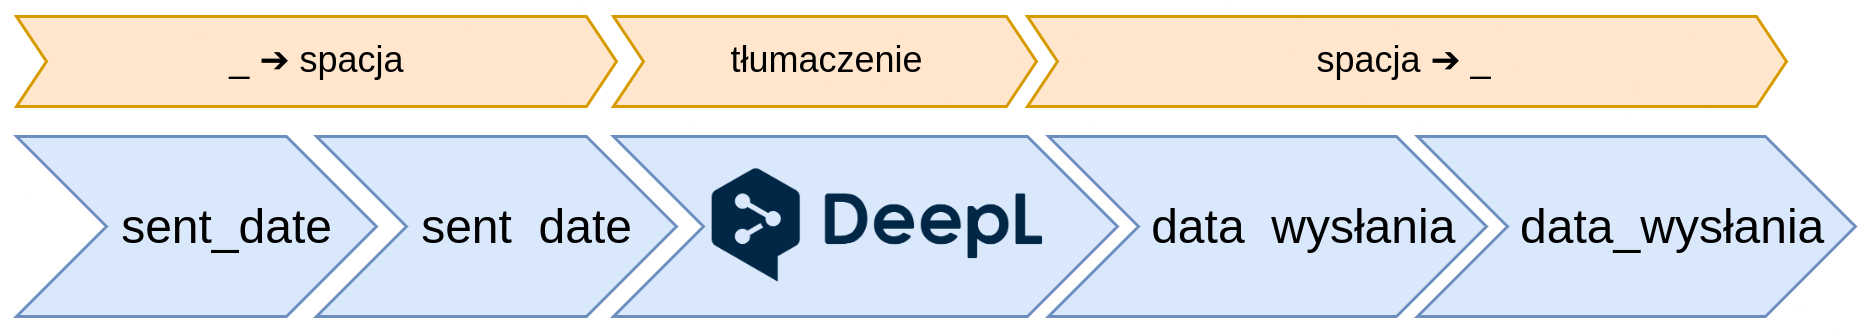
\includegraphics[width=1.0\linewidth]{images/multi_word_translation.png}
  \caption{Schemat algorytmu do tłumaczenia oryginalnych nazw tabel i kolumn}
  \label{fig:multi-word-translation}
\end{figure}

Podstawowa metoda tłumaczenia nazw to ich proste i intuicyjne przekazywanie do tłumacza. Jest to sposób, który został prawdopodobnie wykorzystany we wszystkich tłumaczeniach maszynowych zbioru \code{Spider}, ponieważ ich autorzy nie zwrócili szczególnej uwagi na tę kwestię. Podczas realizacji niniejszej pracy zauważono jednak, że wiele błędów w takich tłumaczeniach wynika z braku uwzględniania przez tłumacza kontekstu i opracowano metodę, która pozwala w dużej mierze obejść ten problem. Dla przykładu kolumna \code{home\_games} podstawową metodą jest tłumaczona jako \code{gry\_domowe}, natomiast ulepszona metoda kontekstowa weźmie pod uwagę, że kolumna ta znajduję się w tabeli \code{stadium} oraz bazie danych \code{game\_injury} i tym razem nazwa zostanie przetłumaczona poprawnie jako \code{mecze\_u\_siebie}.

Metoda kontekstowa polega na prostej obserwacji, że nowoczesne narzędzia bazujące na sieciach neuronowych, w szczególności \code{DeepL}, tłumaczą to samo słowo w różny sposób w zależności od kontekstu, w jakim ono wystąpiło. Z tego powodu do tłumacza poza samymi nazwami tabel i kolumn postanowiono także podawać w roli kontekstu nazwy baz danych, a dla kolumn również nazwy tabel. Zostały opracowane szablony, które służą do tworzenia skontekstualizowanych wyrażeń podawanych do tłumacza i wraz z przykładami użycia zostały przedstawione na rysunku \ref{fig:translation-in-context}. Dla porównania postanowiono dokonać tłumaczenia bezkontekstowego i okazało się, że wynikowe tłumaczenia nazw pomiędzy tymi metodami różnią się dla 21,41\% przypadków, co stanowi dużą różnicę. W tabeli \ref{tab:context-translation-examples} przedstawiono zestawienie kilku nazw przetłumaczonych kontekstowo oraz bezkontekstowo.

\begin{figure}[ht!]
\centering
\begin{subfigure}{0.49\textwidth}
    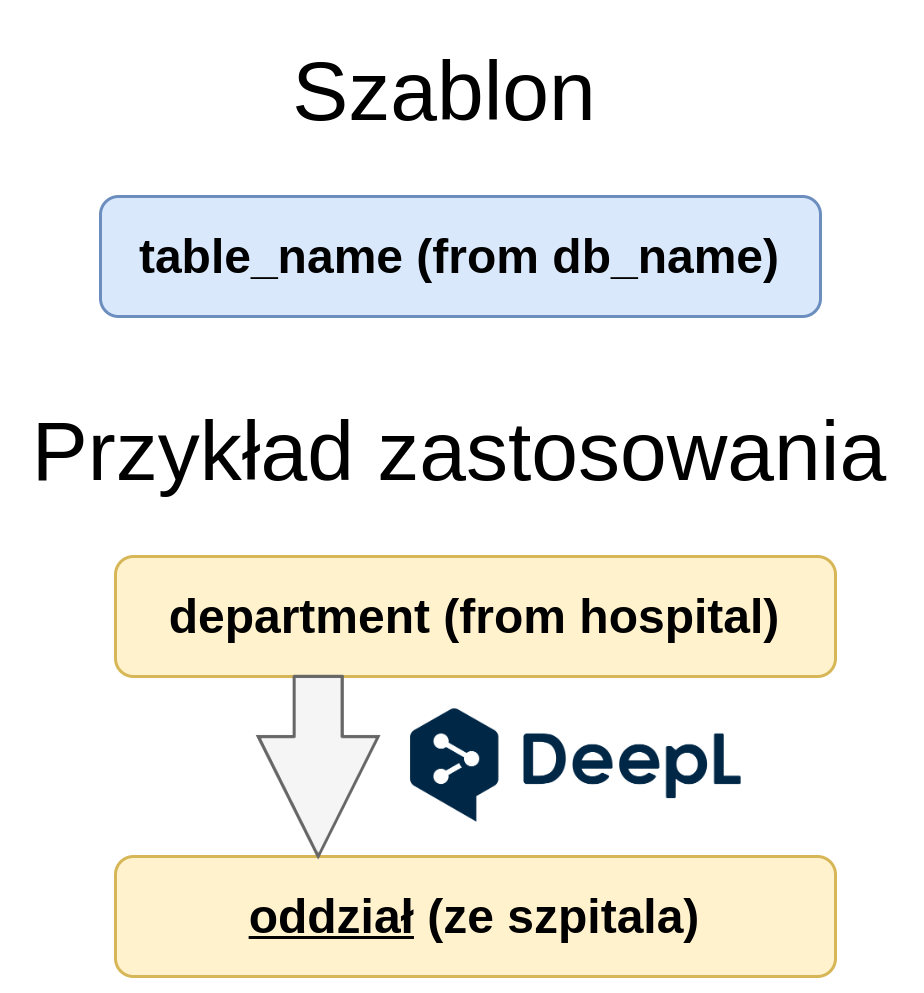
\includegraphics[width=\textwidth]{images/translation_in_context_table.png}
    \caption{Dla tabel}
    \label{fig:first}
\end{subfigure}
\hfill
\begin{subfigure}{0.49\textwidth}
    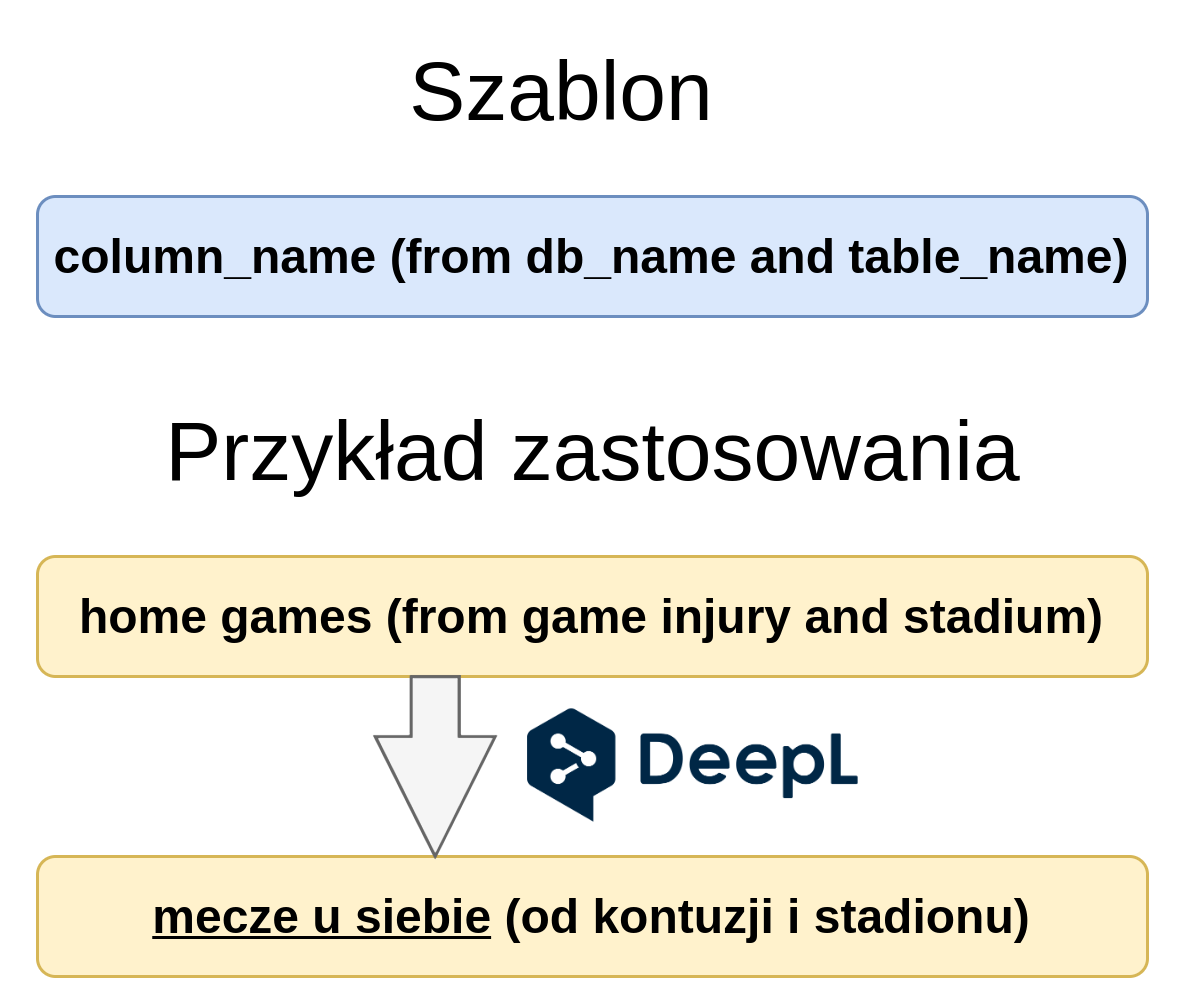
\includegraphics[width=\textwidth]{images/translation_in_context_column.png}
    \caption{Dla kolumn}
    \label{fig:second}
\end{subfigure}
\caption{Szablony do tłumaczenia kontekstowego}
\label{fig:translation-in-context}
\end{figure}

\begin{table}[ht]
    \centering
    \begin{tabular}{|l|l|l|l|l|l|}
        \hline
        \small{\thead{Słowo\\tłumaczone}} &
        \small{\thead{Nazwa\\bazy}} &
        \small{\thead{Czy\\kolumna}} &
        \small{\thead{Nazwa\\tabeli}} & 
        \small{\thead{Tłumaczenie\\bezkontekstowe}} &
        \small{\thead{Tłumaczenie\\kontekstowe}} \\
        \hline
        major & club & tak & student & główny & kierunek \\
        sex & new pets & tak & student & seks & płeć \\
        return data & sakila & tak & rental & data powrotu & data zwrotu \\
        players & wta & nie & --- & gracze & zawodnicy \\
        available policies & insurance fnol & nie & --- & dostępne zasady & dostępne polisy \\
        likes & network & nie & --- & upodobania & polubienia \\
        \hline
    \end{tabular}
    \caption{Porównanie kontekstowego i bezkontekstowego tłumaczenia nazw}
    \label{tab:context-translation-examples}
\end{table}

Przedstawiona strategia tłumaczenia kontekstowego jest zainspirowana metodą \code{SAVe}, opisaną w artykule dotyczącym wielojęzycznego zbioru \code{MultiSpider} \mycite{Dou2022}. Została tam wykorzystana jako metoda augmentacji dla poprawienia osiąganych przez model wyników. Jest bardziej skomplikowana od przedstawionego powyżej wariantu, ponieważ zakłada wykorzystanie wielu szablonów oraz ma dodatkowy etap weryfikacji tłumaczeń, co jednak dla rozważanego problemu nie ma dobrego uzasadnienia.

Oczywistym minusem zaproponowanej metody jest istotne zwiększenie długości tekstów podawanych do tłumacza, co w przypadku \code{DeepL} wpływa na naliczenie wyższych kosztów, czy też szybsze wykorzystanie darmowych limitów -- na co mimo wszystko się zdecydowano. Zaletą strategii kontekstowej jest poprawa tłumaczenia dla wielu nazw, jednak z pewnego punktu widzenia może ona także wpływać na obniżenie czytelności przetłumaczonego schematu. Zdarzają się bowiem przypadki, iż w obrębie jednej bazy danych pewna nazwa kolumny zostaje przetłumaczona na kilka różnych sposobów, chociaż nie powinna. Zmniejsza to spójność tak przetłumaczonego schematu, bo sugeruje, że przechowywane są w tych kolumnach dane o różnym znaczeniu, a w rzeczywistości jest inaczej. Nie jest więc banalnym oszacowanie wypadkowego wpływu zastosowania tej metody na jakość finalnego zbioru, uważa się jednak, że jest on pozytywny.

\subsubsection{Ręczne poprawki}
Po uzyskaniu tłumaczeń maszynowych nazw tabel i kolumn oraz ich wstępnej ocenie stało się oczywiste, że wciąż zawierają pewne błędy. Przejrzenie każdego z nich jedno po drugim wymagałoby znacznego nakładu czasu, więc postanowiono posłużyć się metodami heurystycznymi, by zlokalizować tylko te najbardziej podejrzane tłumaczenia. 

Zauważono, że dla błędnych tłumaczeń bardzo często nazwa przetłumaczona jest identyczna z angielską, więc korzystając z tego faktu, prostych skryptów oraz możliwości edytora \code{Visual Studio Code} dokonano znalezienia właśnie takich przypadków, a następnie je poprawiono. Były to w dużej mierze nazwy składające się z kilku wyrazów połączonych ze sobą za pomocą innej konwencji niż znaki podkreślenia, bo tylko ten najpopularniejszy wariant był obsługiwany w fazie maszynowej. Dość częste były również kilkuliterowe skróty jak \code{mid} (movie id), czy \code{aid} (author id), z którymi -- co nie dziwi -- \code{DeepL} sobie nie poradził. Poza tym dokonano poprawy kilkunastu wyrażeń, w przypadku których zaobserwowano częste pomyłki, jak tłumaczenie \code{name} na \code{imię i nazwisko}, chociaż powinno zostać przetłumaczone jako \code{nazwa}, czy \code{id}, które niepotrzebnie zostało rozwinięte na rozwlekłą nazwę \code{identyfikator}.

Po dokonaniu poprawek związanych z jakością tłumaczeń należało zweryfikować je pod kątem konfliktów nazw. Konieczne było upewnienie się, że w obrębie jednej bazy nie powstało kilka tabel o takich samych nazwach, czy też kilka identycznych kolumn w obrębie tabeli. W tym celu napisano skrypt w języku Python, który analizuje podane mapowanie nazw schematu i raportuje znalezione problemy, które następnie ręcznie naprawiono. Takich konfliktów było zaledwie kilka, lecz ich rozwiązanie okazało się zaskakująco trudne. Dwa przykłady to konflikt nazw kolumn \code{result} i \code{score}, które zostały przetłumaczone jako \code{wynik} oraz tabel \code{Type\_Of\_Restaurant} i \mbox{\code{Restaurant\_Type}}, które zostały przetłumaczone jako \mbox{\code{Typ\_Restauracji}}. W tym drugim przypadku szczególnie trudno było znaleźć dwa różne polskie tłumaczenia i postanowiono zastosować nie do końca satysfakcjonującą parę \code{Typ\_Restauracji} oraz \code{Restauracja\_Typu}.

Na cały etap ręcznych poprawek zostało poświęcone kilka godzin i w jego wyniku zmodyfikowano 10,54\% tłumaczeń maszynowych. Wydaje się to dużą częścią, lecz większość z tych modyfikacji dokonano w szybki, półautomatyczny sposób.


\subsection{Tłumaczenie pytań}
Tłumaczenie pytań sprowadza się do uzupełnienia w przedstawionym wcześniej formacie danych źródłowych atrybutu \code{question.pl} na podstawie \code{question.en}. W tym przypadku pytania zostały bezpośrednio przekazane do tłumacza, bez stosowania żadnych dodatkowych sztuczek. Uznano, że stosowanie tłumaczenia kontekstowego, które oznaczałoby rozszerzenie przekazywanych do tłumacza tekstów o nazwę bazy danych z której pochodzą, nie ma sensu. Wiązałoby się to z tłumaczeniem większej liczby znaków na podstawie których \code{DeepL} obciąża swoich użytkowników, a uzyskana poprawa prawdopodobnie nie byłaby znacząca. Pytania są bowiem zwykle na tyle długie, że pozwalają tłumaczowi na wywnioskowanie domeny, której dotyczą, więc wybranie odpowiednich tłumaczeń dla problematycznych słów nie stanowi już tak dużego problemu.

Etap manualnych poprawek nie został w tym przypadku wykorzystany, gdyż pytania zawierają dużą ilość tekstu i trudno jest dostrzec w nich ewentualne błędy. Nie znaleziono również żadnych sposobów na odszukanie podejrzanych tłumaczeń, czy dokonanie półautomatycznych poprawek, tak jak to miało miejsce dla tłumaczenia nazw tabel i kolumn. Ostatecznie maszynowe tłumaczenia pytań wydawały się na tyle wysokiej jakości, że postanowiono przejść do kolejnych etapów.

\subsection{Tłumaczenie wartości w zapytaniach SQL}
Tłumaczenie wartości w zapytaniach SQL odbywa się poprzez uzupełnienie atrybutu \code{query.pl} na podstawie \code{query.en} w pliku danych źródłowych. Ten ostatni atrybut zawiera oryginalne zapytania SQL, natomiast pierwszy zapytania z wszelkimi anglojęzycznymi łańcuchami znaków przetłumaczonymi na język polski.

W celu znalezienia w danym zapytaniu wartości tekstowych dokonywano jego przetwarzania z wykorzystaniem biblioteki \code{sqlparse}. Pozwalała ona podzielić zapytanie na poszczególne tokeny i wybrać te, które posiadają typ \code{Token.Literal.String}, czyli stanowią wartości tekstowe. Są to wyrażenia zapisane się w cudzysłowach, które przekazywano do \code{DeepL} w celu uzyskania tłumaczeń, a następnie zastępowano nimi oryginalne teksty. Wyjątek stanowią wartości występujące w roli szablonów po słowie kluczowym \code{LIKE}, takie jak \code{'\%Hey\%'}, \code{'\%East\%'}, \code{'S\%'}. Nie są zapisane w języku naturalnym, ponieważ zawierają specjalne znaki, stanowiące problem dla tłumacza maszynowego. Biorąc pod uwagę rzadkość takich przypadków, postanowiono przetłumaczyć je manualnie. Wizualizacja tego etapu została przedstawiona na rysunku \ref{fig:value-translation}.

\begin{figure}[ht!]
  \centering
  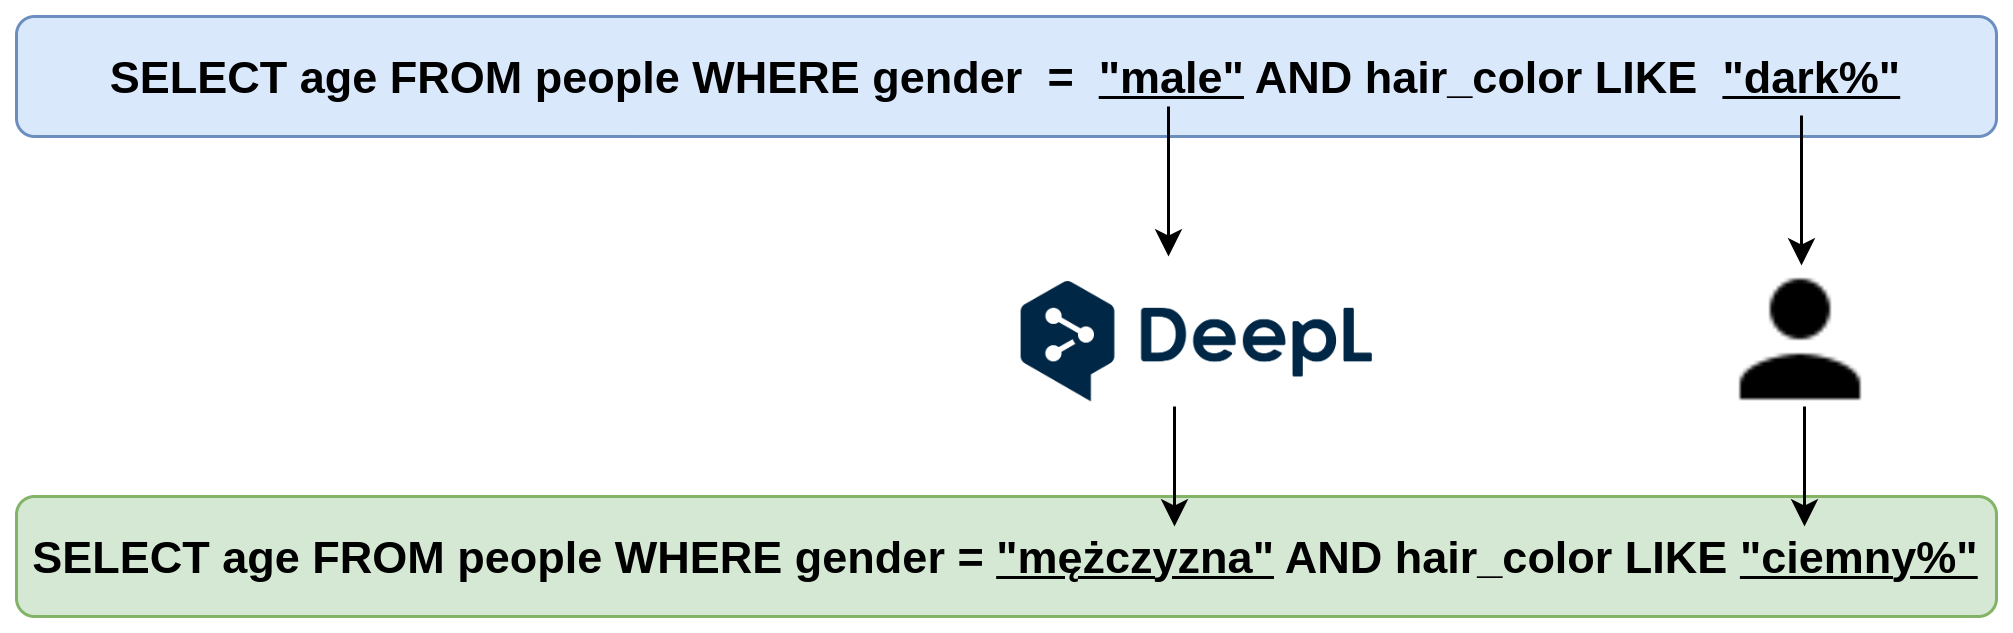
\includegraphics[width=1.0\linewidth]{images/value_translation.png}
  \caption{Wizualizacja etapu tłumaczenia wartości w zapytaniach SQL}
  \label{fig:value-translation}
\end{figure}

\section{Stworzone zbiory}
Niniejszy część stanowi ukoronowanie pracy nad polskimi zbiorami danych, ponieważ zawiera ich ostateczne przedstawienie wraz 
z analizą. Zgodnie z obraną strategią kompletne zbiory stanowią połączenie jednego z bazowych zbiorów oraz jednego z mapowań nazw tabel i kolumn, dlatego komponenty te zostaną opisane osobno. Na koniec kilka ich połączeń zostanie nazwanych w celu ułatwienia dalszych rozważań.

\subsection{Zbiory bazowe}
Przygotowanych zostało pięć bazowych zbiorów, z których zdecydowanie najistotniejszym ze względu na swoją renomę oraz powszechne wykorzystanie jest \code{Spider}. W celu weryfikacji i porównywania trenowanych modeli przetłumaczone zostały także zbiory \code{Spider-DK} oraz \code{Spider-Syn}. \code{CoSQL} oraz \code{SParC} to natomiast znacznie różniące się od swoich oryginałów zbiory, które przygotowano i przetłumaczono głównie w celu uzyskania dodatkowych danych treningowych.

\begin{table}[ht]
    \centering
    \begin{tabular}{|l|R{0.15\textwidth}|R{0.15\textwidth}|R{0.15\textwidth}|}
        \hline
        \thead{Zbiór} & \thead{Część\\treningowa} & \thead{Część\\walidacyjna} & \thead{Razem} \\
        \hline
        Spider & 8659 & 1034 & 9693 \\
        Spider-Syn & 3556 & 773 & 4329 \\
        Spider-DK & 0 & 535 & 535 \\
        CoSQL & 1562 & 230 & 1792 \\
        SParC & 2651 & 366 & 3017 \\
        \hline
        Razem & 16428 & 2938 & 19366 \\
        \hline
    \end{tabular}
    \caption{Zestawienie liczby próbek w poszczególnych zbiorach}
    \label{tab:samples-count}
\end{table}

W tabeli \ref{tab:samples-count} przedstawione zostały liczności próbek we wszystkich stworzonych zbiorach bazowych z uwzględnieniem podziału na części treningowe oraz walidacyjne. \code{Spider} to zbiór najliczniejszy, z którego żadne próbki nie były usuwane i dokładnie odpowiadają oryginalnym. Drugim największym jest \code{Spider-Syn}, który zawiera przykłady ze \code{Spider} z niewielkimi modyfikacjami, lecz w wyniku usuwania duplikatów skurczył się o ponad połowę. Zbiory \code{SParC} oraz \code{CoSQL} są następne w kolejności i one również w czasie deduplikacji zostały uszczuplone. Najmniejszym zbiorem, posiadającym jedynie część walidacyjną, jest \code{Spider-DK}, chociaż z niego żadne próbki usuwane nie były.

\begin{table}[ht]
    \centering
    \begin{tabular}{|l|R{0.15\textwidth}|R{0.15\textwidth}|R{0.15\textwidth}|R{0.15\textwidth}|R{0.15\textwidth}|}
        \hline
        \thead{Zbiór} & \thead{Easy} & \thead{Medium} & \thead{Hard} & \thead{Extra Hard} \\
        \hline
        Spider & 2231 (23\%) & 3445 (36\%) & 2095 (22\%) & 1922 (20\%) \\
        Spider-DK & 110 (21\%) & 246 (46\%) & 74 (14\%) & 105 (20\%) \\
        Spider-Syn & 952 (22\%) & 1825 (42\%) & 884 (20\%) & 668 (15\%) \\
        CoSQL & 949 (53\%) & 488 (27\%) & 222 (12\%) & 133 (\s7\%) \\
        SParC & 2131 (71\%) & 706 (23\%) & 138 (\s5\%) & 42 (\s1\%) \\
        \hline
        Wszystkie & 6373 (33\%) & 6710 (35\%) & 3413 (18\%) & 2870 (15\%) \\
        \hline
    \end{tabular}
    \caption{Zestawienia liczby próbek o poszczególnych poziomach trudności}
    \label{tab:difficulty}
\end{table}

Repozytorium zbioru \code{Spider} \mycite{spider-repo} dostarcza algorytm pozwalający przypisać do każdego zapytania SQL jeden z czterech poziomów trudności: \code{Easy}, \code{Medium}, \code{Hard} oraz \code{Extra Hard}. Odbywa się to poprzez zliczenie w zapytaniu różnych komponentów i klasyfikację na podstawie zdefiniowanych reguł. Przykłady zapytań o poszczególnych poziomach trudności przedstawiono na rysunku \ref{fig:sql-difficulties}. Postanowiono dokonać analizy rozłożenia zapytań o poszczególnych poziomach trudności we wszystkich zbiorach. Wyniki tej analizy umieszczono w tabeli \ref{tab:difficulty}. Można je podsumować twierdzeniem, że najbardziej skomplikowane zapytania występują w zbiorze \code{Spider}, co niewątpliwie jest istotnym powodem jego popularności. Niemal równie trudne zapytania posiada zbiór \code{Spider-DK}, lecz jest on wielokrotnie mniejszy. Z drugiej strony wyjątkowo proste okazały się zapytania znajdujące w zbiorach \code{CoSQL} oraz \code{SParC}.

\begin{table}[ht]
    \centering
    \begin{tabular}{|l|r|r|}
        \hline
        \thead{Zbiór} & \thead{Pytania (en / pl)} & \thead{Wartości (en / pl)} \\
        \hline
        Spider & 66,74 / 66,44 & 10,66 / 11,28 \\
        Spider-DK & 66,01 / 65,93 & \s8,47 / \s8,59 \\
        Spider-Syn & 74,03 / 74,14 & 9,65 / 10,28 \\
        CoSQL & 53,05 / 52,66 & 10,11 / 10,72 \\
        SParC & 44,94 / 45,52 & 10,24 / 10,84 \\
        \hline
        Wszystkie & 63,69 / 63,61 & 10,32 / 10,94 \\
        \hline
    \end{tabular}
    \caption{Zestawienie średniej liczby znaków w pytaniach i wartościach}
    \label{tab:questions-lengths}
\end{table}

Interesującą analizą jest zestawienie długości tekstów angielskich oraz przetłumaczonych na język polski. Zgodnie z danymi ukazanymi w tabeli \ref{tab:questions-lengths} średnie długości wszystkich pytań liczone w znakach różnią się zaledwie o 0,08. W przypadku długości wartości tekstowych różnica ta jest nieco większa i wynosi 0,61. Wzrost może być spowodowany faktem, że występują one jedynie w niektórych próbkach i ze statystycznego punktu widzenia liczba ta jest mniej pewna. Mimo wszystko różnice okazały się zdecydowanie mniejsze od spodziewanych. Oznacza to, że długość pytań i wartości nie będzie miała wpływu na utrudnienie, czy też ułatwienia tłumaczenia zapytań w stosunku do języka angielskiego.

\begin{figure}[ht]
\begin{tabular}{cc}
\begin{subfigure}{0.48\textwidth}
    \begin{minipage}{\linewidth}
        \lstinputlisting[
        style=sql,
        numbers=none,
        showlines=true,
        nolol,
        ]{listings/difficulties/easy.sql}
    \end{minipage}
    \caption{Easy}
\end{subfigure}
&
\begin{subfigure}{0.48\textwidth}
    \begin{minipage}{\linewidth}
        \lstinputlisting[
        style=sql,
        numbers=none,
        showlines=true,
        nolol,
        ]{listings/difficulties/medium.sql}
    \end{minipage}
    \caption{Medium}
\end{subfigure}
\\
  \begin{subfigure}{0.48\textwidth}
    \begin{minipage}{\linewidth}
        \lstinputlisting[
        style=sql,
        numbers=none,
        showlines=true,
        nolol,
        ]{listings/difficulties/hard.sql}
    \end{minipage}
    \caption{Hard}
\end{subfigure}
&
\begin{subfigure}{0.48\textwidth}
    \begin{minipage}{\linewidth}
        \lstinputlisting[
        style=sql,
        numbers=none,
        showlines=true,
        nolol,
        ]{listings/difficulties/extra.sql}
    \end{minipage}
    \caption{Extra Hard}
\end{subfigure}
\end{tabular}
\caption{Przykłady zapytań SQL o różnych poziomach trudności}
\label{fig:sql-difficulties}
\end{figure}

\subsection{Mapowania nazw}
Zgodnie z przedstawionymi wcześniej informacjami opracowane zostały dwie główne drogi dokonywania tłumaczeń nazw tabel i kolumn: metoda bezkontekstowa oraz uważana za lepszą metoda kontekstowa. Mapowania nazw uzyskane z wykorzystaniem tych strategii nazwano odpowiednio \code{pl\_nocontext} oraz \code{pl\_context}. W tłumaczeniach maszynowych powstałych metoda kontekstową dokonano następnie dużej liczby półautomatycznych poprawek i stworzone w ten sposób mapowanie nazwano \code{pl\_context\_curated}. Przewidziano również mapowanie zachowujące oryginalne, angielskie nazwy, które określono jako \code{en\_original}.

Wymienione mapowania zawierają polskie znaki, które jednak rzadko są spotykane w praktyce, więc opracowano skrypt, który dokonuje ich zastąpienia występującymi w kodowaniu \code{ASCII} odpowiednikami, jak \code{wysokość -> wysokosc}. W ten sposób powstały odpowiadające trzem wcześniej wspomnianym mapowania z sufiksem \code{\_sanitized}. Schemat przedstawiający naszkicowane zależności został przedstawiony na rysunku \ref{fig:mappings}.

\begin{figure}[ht!]
  \centering
  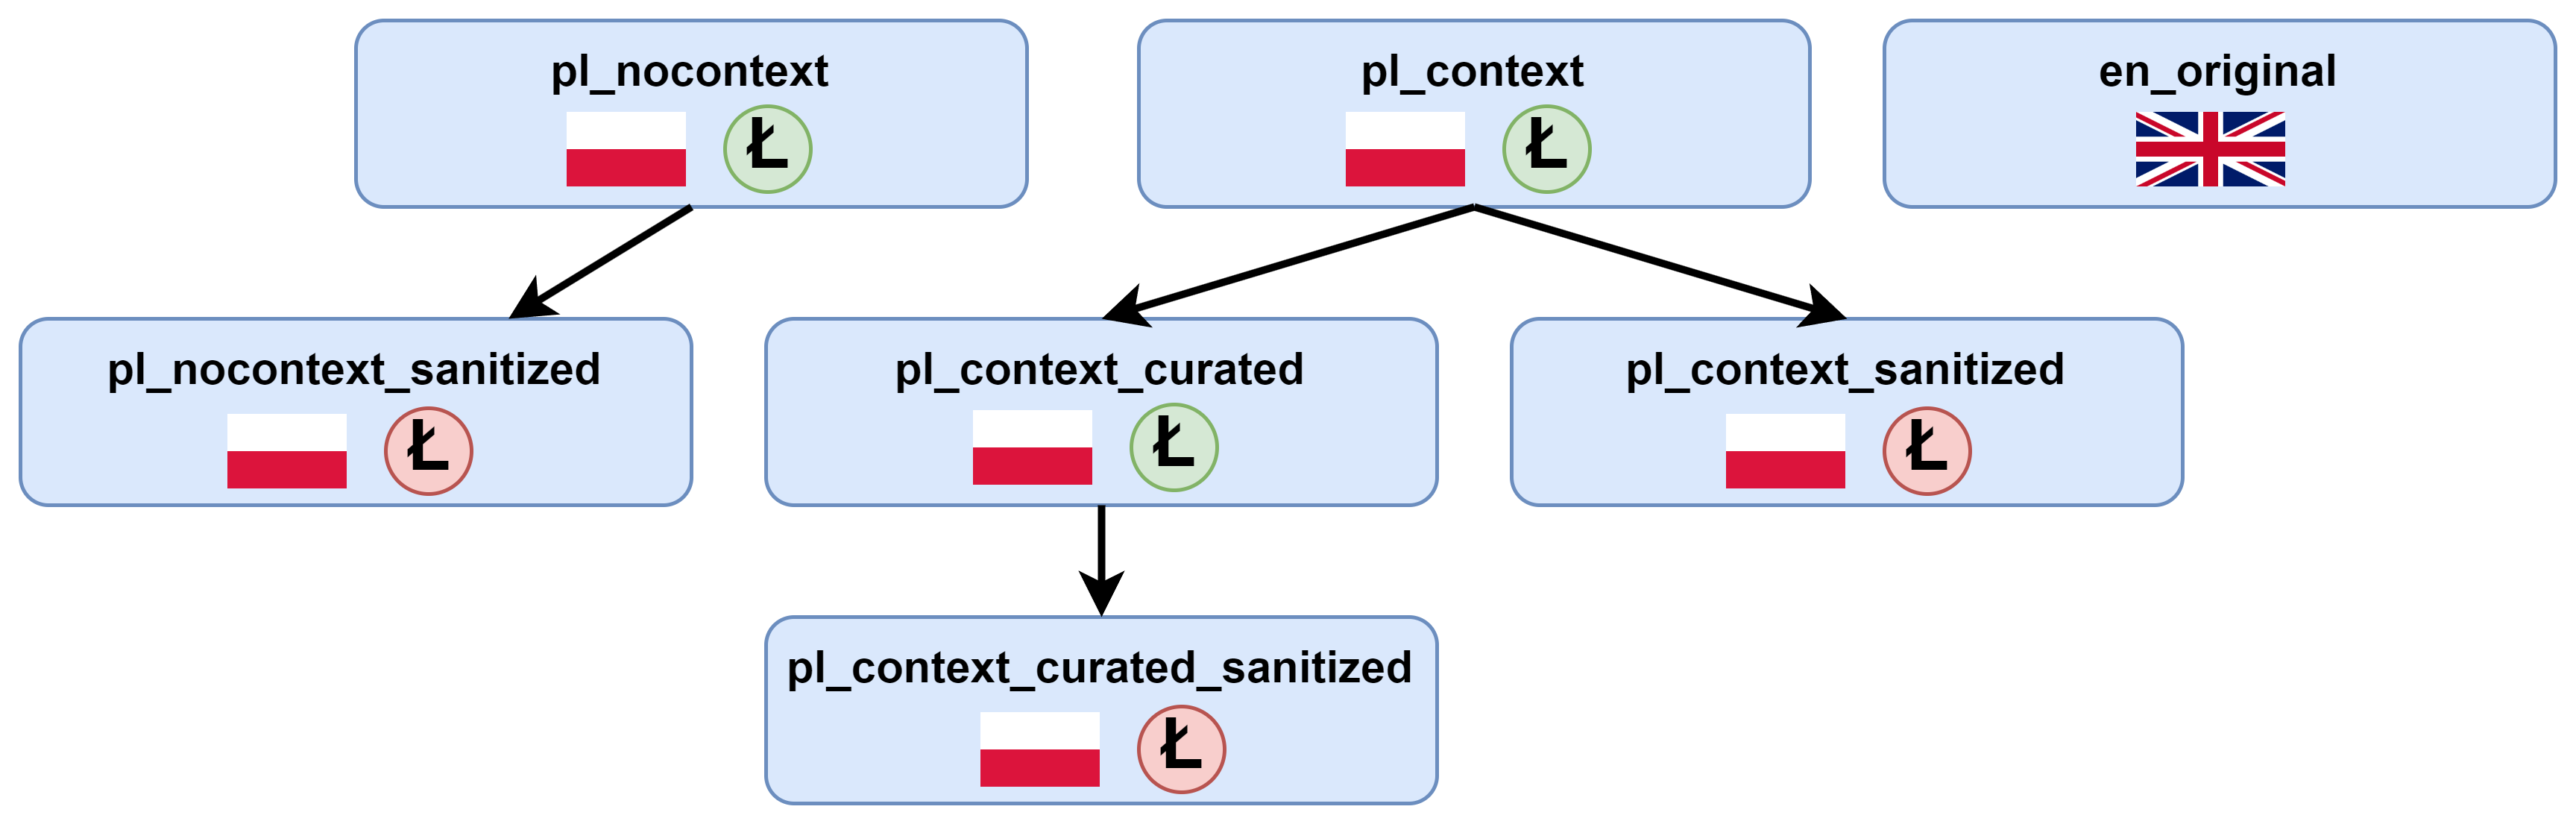
\includegraphics[width=1.0\linewidth]{images/mappings.png}
  \lcaption{Schemat zależności pomiędzy stworzonymi mapowaniami nazw}{Litera Ł w zielonym kółku oznacza obecność polskich znaków, natomiast w czerwonym ich brak.}
  \label{fig:mappings}
\end{figure}

Podobnie jak to było w przypadku pytań, tutaj również postanowiono zbadać, w jaki sposób zastosowanie poszczególnych mapowań wpływa na długość finalnych nazw tabel i kolumn. Wyniki tej analizy przedstawiono w tabeli \ref{tab:names-lengths}. Można zauważyć, że tłumaczenie na język polski zwiększa długości o około jeden znak, co stanowi prawie 10\%. Jest to znaczny wzrost, biorąc pod uwagę, że w przypadku tłumaczenia pytań był on marginalny. Wyjaśniać może to obserwacja, że angielskie nazwy tabel i kolumn często bywają zapisywane skrótowo, a tłumaczenia produkowane przez \code{DeepL} są bardziej opisowe. Przykładowo nazwa tabeli \code{Student\_Tests\_Taken} została przetłumaczona jako \code{Testy\_Wykonane\_Przez\_Uczniów}.

\begin{table}[ht]
    \centering
    \begin{tabular}{|l|c|c|c|c|}
        \hline
        \multirow{2}{*}[-6pt]{\thead{Nazwy mapowań}} &
        \multicolumn{2}{c|}{\thead{Tabele}} &
        \multicolumn{2}{c|}{\thead{Kolumny}} \\
        \cline{2-5}
        \multirow{2}{*}{} &
        \thead{Nazwy\\naturalne} &
        \thead{Nazwy\\oryginalne} &
        \thead{Nazwy\\naturalne} &
        \thead{Nazwy\\oryginalne} \\
        \hline
        \code{en\_original} & 10,48 & 10,28 & 10,26 & \s9,87 \\
        \code{pl\_nocontext} & 11,37 & 11,17 & 11,24 & 10,83 \\
        \code{pl\_context } & 11,46 & 11,23 & 11,38 & 11,11 \\
        \code{pl\_context\_curated} & 11,55 & 11,29 & 11,36 & 11,07 \\
        \hline
    \end{tabular}
    \caption{Zestawienie średniej liczby znaków w mapowaniach nazw}
    \label{tab:names-lengths}
\end{table}

\subsection{Nazwane warianty}

W celu ułatwienia dalszej pracy poprzez możliwość odwoływania się do konkretnych zbiorów kilka ich konfiguracji zostało nazwanych. Ponadto zdefiniowane zostały pewne połączenia tych zbiorów, ponieważ występują do nich częste odwołania.

\begin{figure}[ht!]
  \centering
  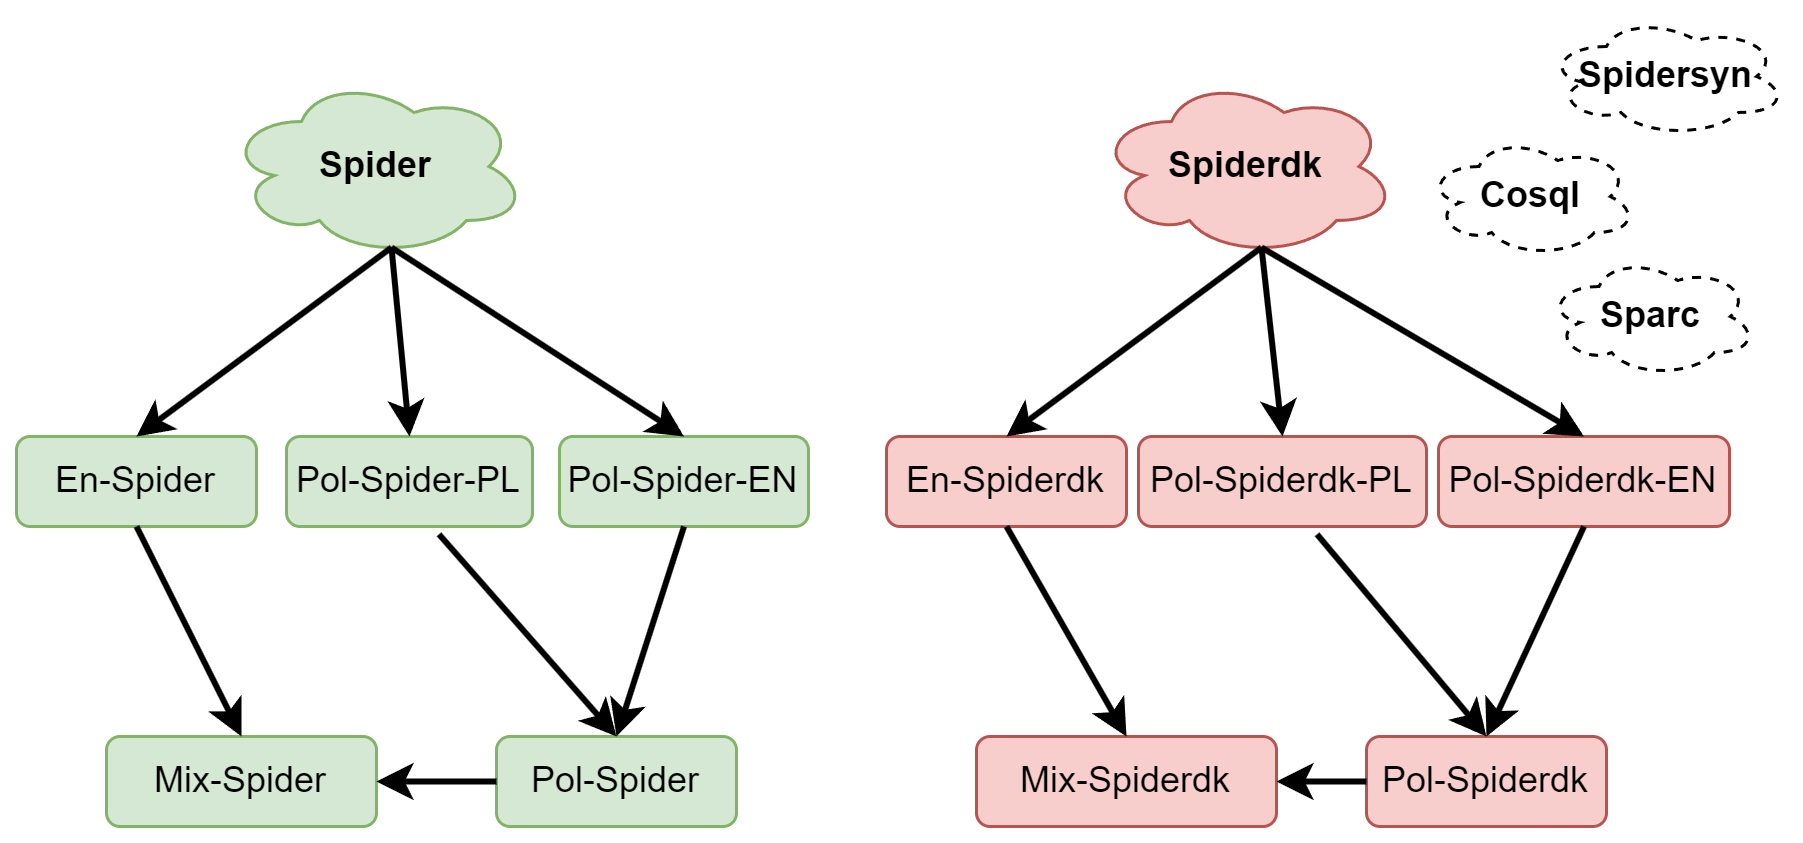
\includegraphics[width=1.0\linewidth]{images/datasets.png}
  \caption{Schemat zależności pomiędzy zbudowanymi zbiorami danych}
  \label{fig:datasets}
\end{figure}

Schemat zdefiniowanych zbiorów został przedstawiony na rysunku \ref{fig:datasets}. Można z niego odczytać, że na bazie zbioru \code{Spider} wygenerowane zostały trzy zbiory pochodne. \code{En-Spider} to wariant całkowicie angielski, bardzo podobny do oryginalnego \code{Spider}, ale z minimalnymi różnicami, jak sposób tokenizacji. Wykorzystuje angielskie pytania i wartości oraz mapowanie \code{en\_original}. Kolejny to \code{Pol-Spider-PL}, czyli wariant polski, z polskim schematem baz danych, uzyskanym za pomocą mapowania \code{pl\_context\_curated\_sanitized}. Trzecim jest natomiast \mbox{\code{Pol-Spider-EN}}, czyli również zbiór polski, ale z angielskim schematem baz danych, stworzonym za pomocą mapowania \code{en\_original}.

Opracowany został dodatkowo skrypt, który pozwala na łatwe łączenie zbiorów. Za jego pomocą dokonano połączenia dwóch wspomnianych polskich wariantów w zbiór, który nazwano \code{Pol-Spider}. Ma on podwójny rozmiar i obejmuje dwojaki sposób nazewnictwa kolumn i tabel. Jest istotny z praktycznego punktu widzenia, ponieważ nie ogranicza się tylko do pierwszego, czy drugiego przypadku, lecz obejmuje obie powszechnie spotykane konwencje. Po rozszerzeniu tego już rozbudowanego polskiego zbioru o angielski \code{En-Spider} powstaje natomiast \code{Mix-Spider}, czyli dość nietypowy zbiór zawierający próbki w obu językach.

Podobny schemat nazewnictwa do przedstawionego powyżej został zastosowany do reszty zbiorów bazowych, czyli \code{Spider-DK}, \code{Spider-Syn}, \code{CoSQL} oraz \code{SParC}. Wykorzystano wymowne i schematyczne nazwy, aby ułatwić ich zapamiętanie. Możliwych do wygenerowania konfiguracji zbiorów jest znacznie więcej, lecz do tych przedstawionych powyżej będą występowały częstsze odwołania w dalszej części pracy.
